\documentclass{article}
\usepackage{graphicx,amsmath, mathtools, amssymb, fancyhdr, xcolor, float} % Required for inserting images

\graphicspath{{Images/}}

\setlength{\oddsidemargin}{0in}
\setlength{\textwidth}{6.5in}
\setlength{\topmargin}{-.55in}
\setlength{\textheight}{9in}
\pagestyle{fancy}

\fancyfoot{}
\fancyhead[R]{\thepage}
\fancyhead[L]{MAE 5131}


\begin{document}

\begin{center}
    {\huge CFD Homework 3}
    \vspace{0.5cm}

    {\large Michael Nameika}
    \vspace{0.5cm}
\end{center}

\begin{itemize}
    \item[\textbf{1}.] Consider a viscous Burger's equation (convection-diffusion equation).
    \[\frac{\partial u}{\partial t} + c\frac{\partial u}{\partial x} = \mu\frac{\partial^2u}{\partial x^2}\]
    subject to periodic boundary conditions:
    \[u(L,t) = u(0,t)\]
    and the initial condition:
    \[u(x,0) = A\sin(2\pi k x)\]
    in which $A = 1$.
    \newline\newline
    The analytical solution is a decaying traveling wave in the following form
    \[u(x,t) = e^{-\mu 4\pi^2k^2t}\sin(2\pi k(x - ct)).\]
    The diffusion coefficient $\mu = 0.05$, $c = 1$, $k = 1$, and $L = 1$.
    \newline\newline
    \textbf{Objective:} We will study the effect of time step $\Delta t$ and spatial resoultion $\Delta x$ using the FTCS (forward in time central difference in space). The numerical solution in the following problems are taken at $t = 0.5$. Here in the code, we specify the periodic boundary condition ($N$ is the index of the last node, i.e., $x(N) = L$). As shown in the following figure, $u_1 = u_N$, $u_2 = u_{N+1}$, $u_0 = u_{N-1}$. Note here $u_0$ and $u_{N-1}$ do not really exist, putting there just for explanation of periodic boundary condition. We can start from
    \[u_{N}^{n + 1} = u_N^n - \frac{\Delta t}{2\Delta x}c(u^n_{\color{red} N+1} - u_{N-1}^n) + \frac{\Delta t}{(\Delta x)^2}\mu(u^n_{\color{red} N+1} - 2u_N^n + u_{N-1}^n).\]
    But since $u_{N+1}$ does not exist, and $u_2 = u_{N+1}$, we then have:
    \[u_{N}^{n + 1} = u_N^n - \frac{\Delta t}{2\Delta x}c(u^n_{\color{red} 2} - u_{N-1}^n) + \frac{\Delta t}{(\Delta x)^2}\mu(u^n_{\color{red} 2} - 2u_N^n + u_{N-1}^n)\]
    \[u_1^{n+1} = u_{N}^{n+1}.\]
    Define the error as $\varepsilon = \Delta x\sqrt{\displaystyle \sum_{i = 1}^N (u_i - u_{\text{exact}})^2 }$, note this definition is so called $\ell^2$ error norm.
    \begin{itemize}
        \item[(1)] Test different $\Delta t$. Use $N = 21$, $\Delta t = 0.05$, $\Delta t = 0.025$, $\Delta t = 0.0125$, $\Delta t = 0.0005$, obtain the simulation result from FTCS, calculate the error and plot $\varepsilon$ versus $\Delta t.$ Also, plot $u(i)$ versus $x$ with $\Delta t$ as a parameter, and the exact solution $u(x)$ versus $x$. 
        \newline\newline
        \textit{Soln.} For this problem, I set the final time to be $t = 1$. To implement the periodic boundary conditions, it is equivalent to uniformly discretize the domain $x \in [0,1]$ and delete the last point to avoid double counting and implement the spatial finite difference schemes in the following way. Let $D_1, D_2$ be the differentiation matrices for the the centered difference scheme for the first and second derivative, respectively. Then
        \begin{align*}
            D_1 &= \frac{1}{2\Delta x}\begin{pmatrix}
                0 & 1 &  &  &  & -1\\
                -1 & 0 & 1 &  &  & \\
                 & -1 & 0 & 1 &  & \\
                 & & \ddots & \ddots & \ddots &\\
                 &  & & -1 & 0 & 1\\
                1 &  &  & & -1 & 0
            \end{pmatrix}\\
            D_2 &= \frac{1}{\Delta x^2}\begin{pmatrix}
                -2 & 1 & & & & 1\\
                1 & -2 & 1 & & & \\
                & 1 & -2 & 1 & & \\
                & & \ddots & \ddots & \ddots & \\
                & & & 1 & -2 & 1\\
                1 & & & & 1 & -2
            \end{pmatrix}.
        \end{align*}
        where $D_1,D_2$ are $(N_x - 1) \times (N_x - 1)$ matrices. In implementation, at each time step, we perform the following update:
        \[u^{i + 1} = u^i - cD_1u^i + \mu D_2u^i.\]
        Implementing this, we find the following for various values of $\Delta t$:

        
        \begin{figure}[H]
            \begin{center}
                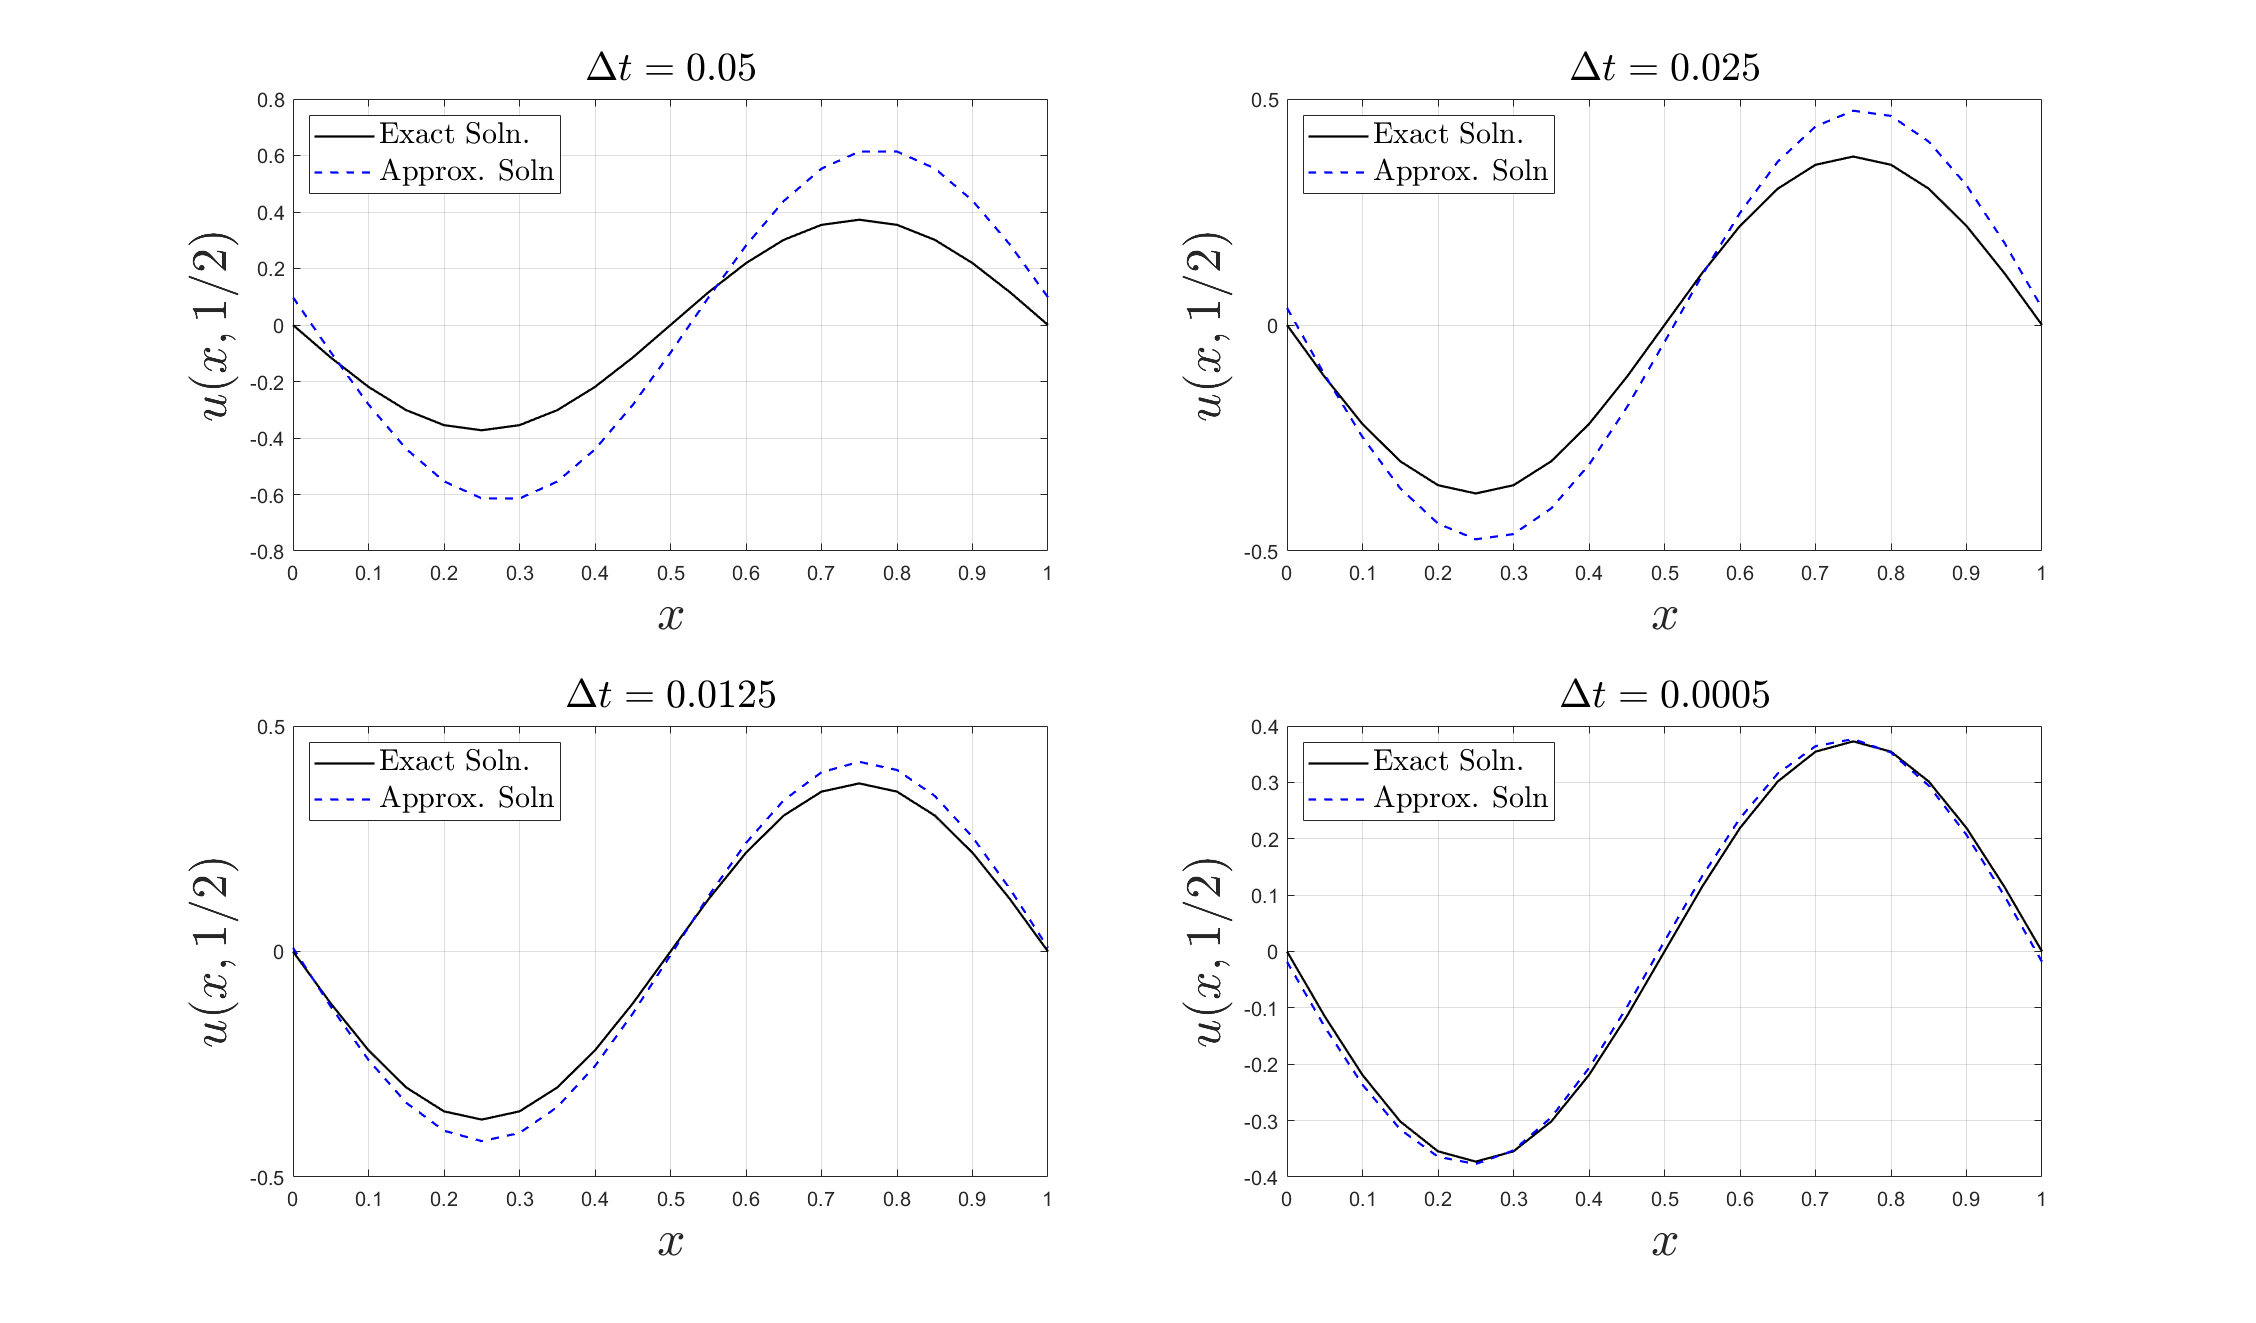
\includegraphics[scale = 0.25]{prob_1_subplots.png}
                \newline
                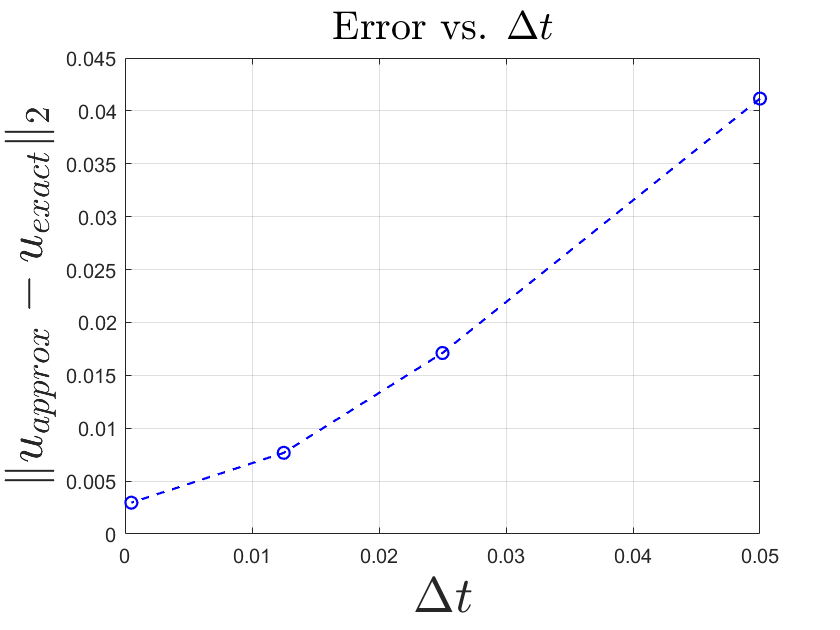
\includegraphics[scale = 0.3]{err_vs_dt_prob1_1.png}
            \end{center}
        \end{figure}


        \item[(2)] Effect of spatial resolution. Take $\Delta t = 0.0005$, use different meshes $N = 9$, $N = 17$, $N = 33$, $N = 65$, $N = 129$, $N = 257$, calculate the numerical results using FTCS.
        \newline
        If the error $\varepsilon$ is of the second order, then $\varepsilon$ can be written as: $\varepsilon = Coeff \cdot (\Delta x)^2$. Take log, we have
        \[\log_{10}(\varepsilon) = \log_{10}(Coeff) - 2\log_{10}(1/\Delta x)\]
        Plot $\log_{10}(\varepsilon)$ versus $\log_{10}(1/\Delta x)$, and check if the slope is around $-2$. Plot $u(i)$ versus $x$ with $N$ as a parameter, and the exact solution $u(x)$ versus $x$.
        \newline\newline
        \textit{Soln.} Again running the simulation to the final time of $t = 1$, we find the following plots for the numerical and exact solutions to the problem. We note that for the case $N_x = 257$, we found that our numerical solution diverged, which we plot separately and exclude the error from the error plot. Note that in the error plot, we do see the error approximately has slope of $-2$ on the log-log plot.
        \begin{figure}[H]
            \begin{center}
                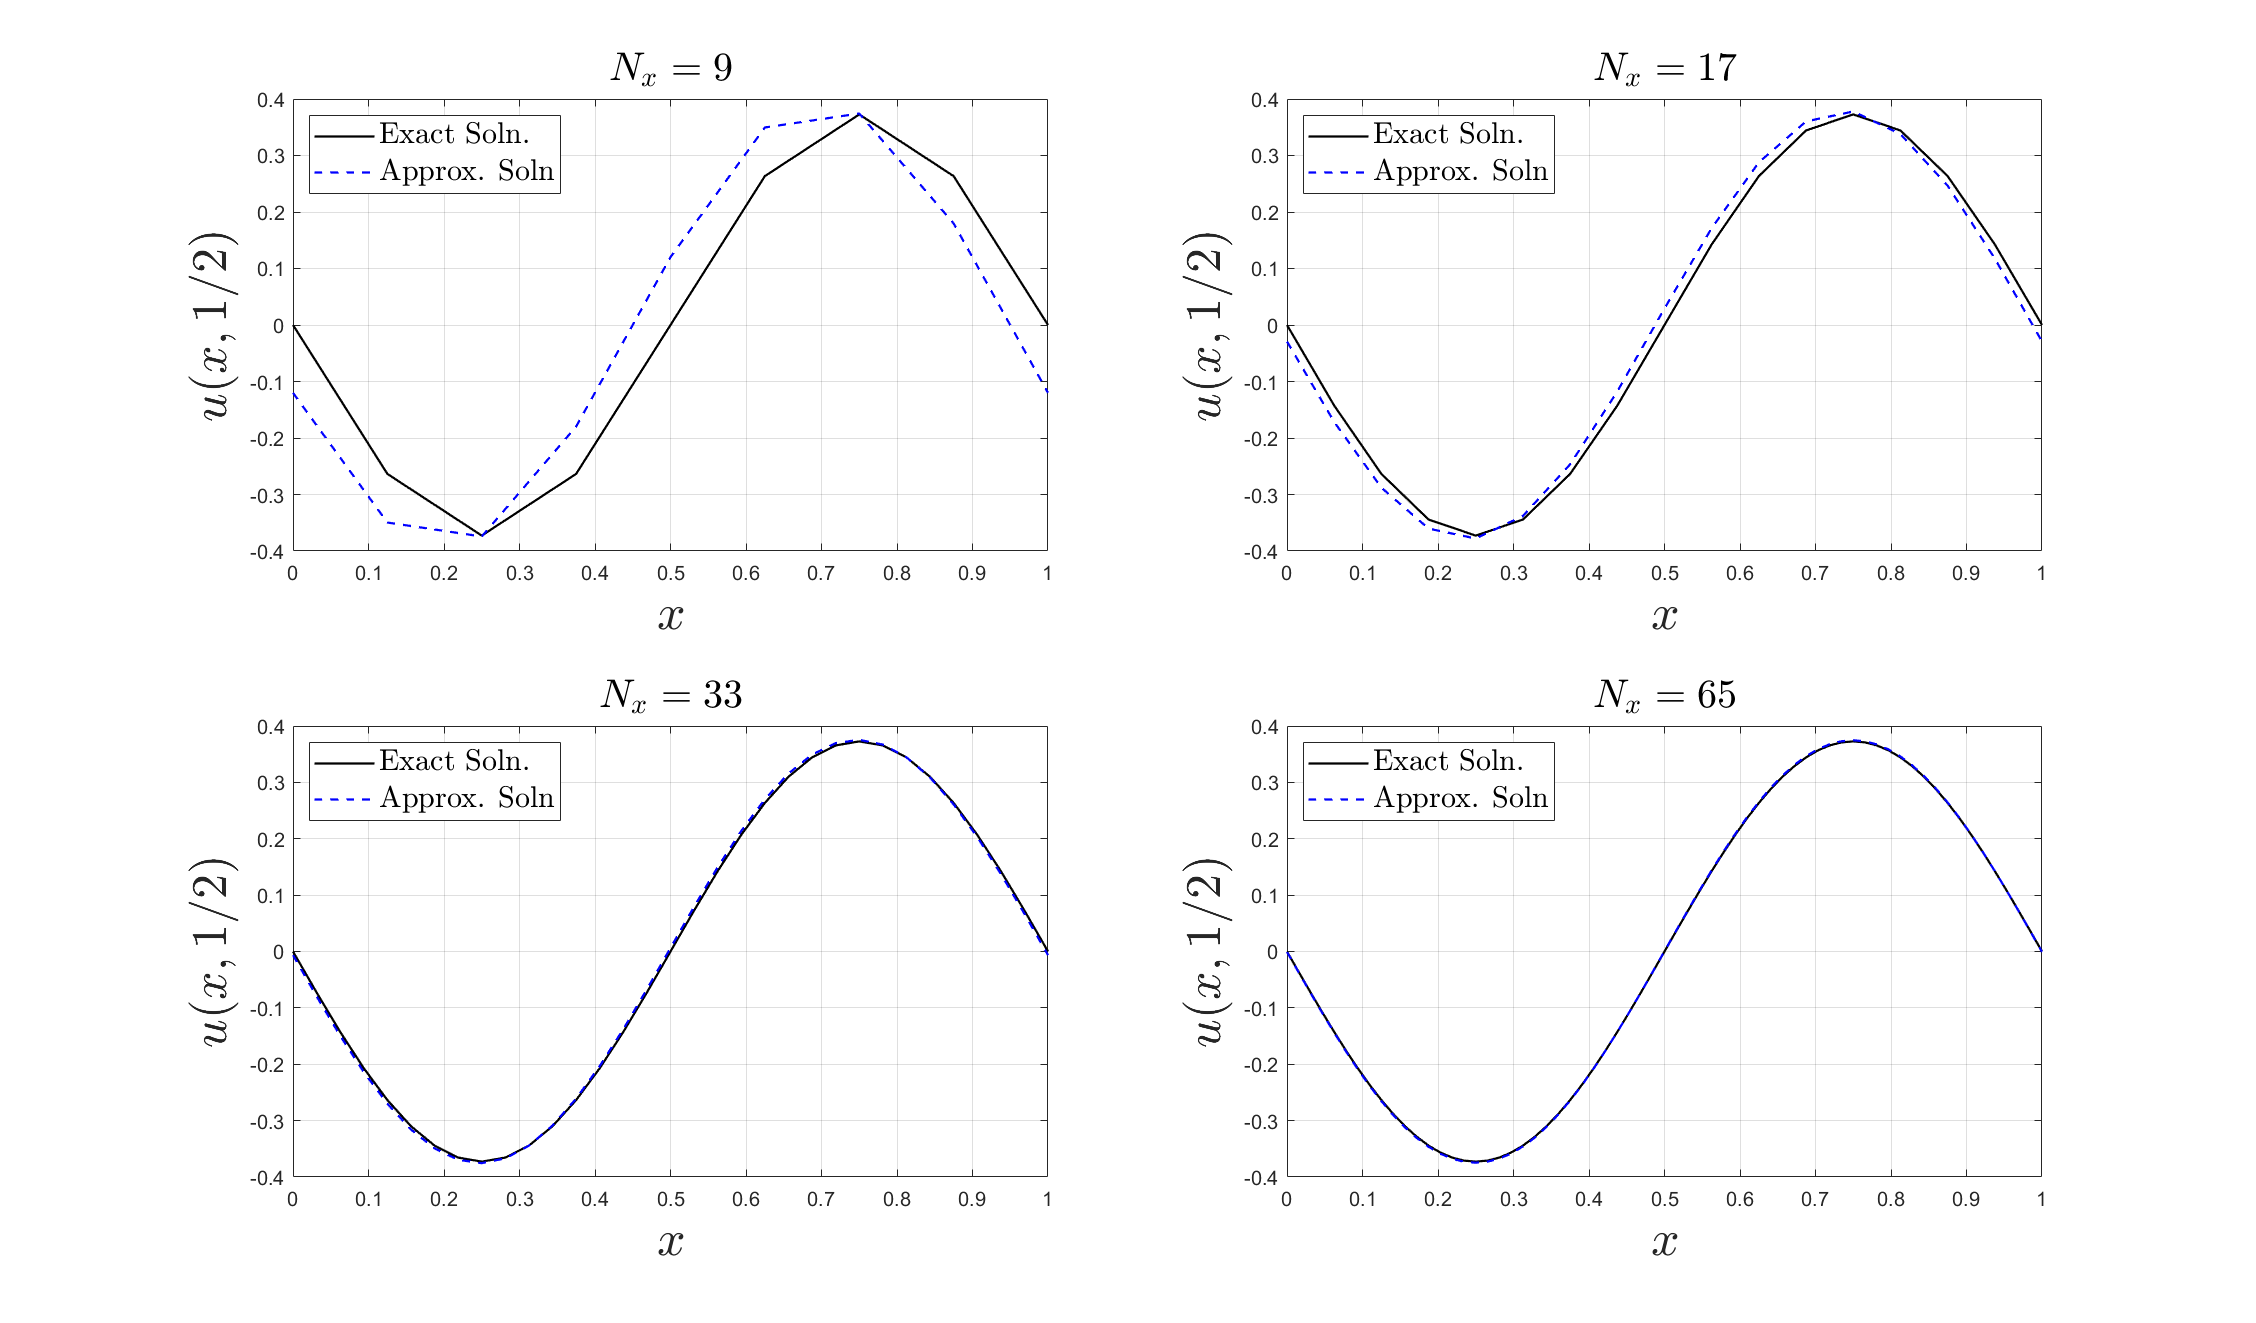
\includegraphics[scale = 0.25]{prob_1_2_subplots.png}
                \newline
                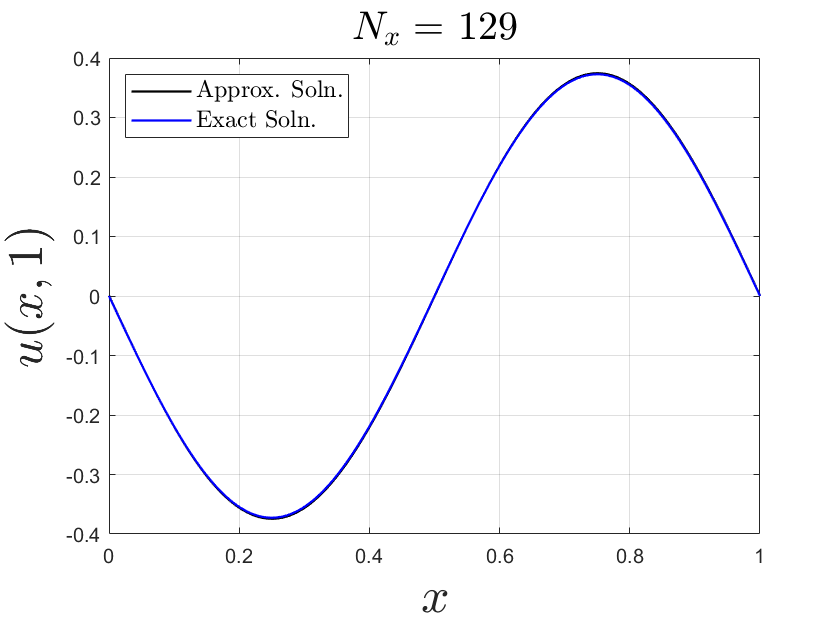
\includegraphics[scale = 0.3]{prob_1_2_nx_129.png}
                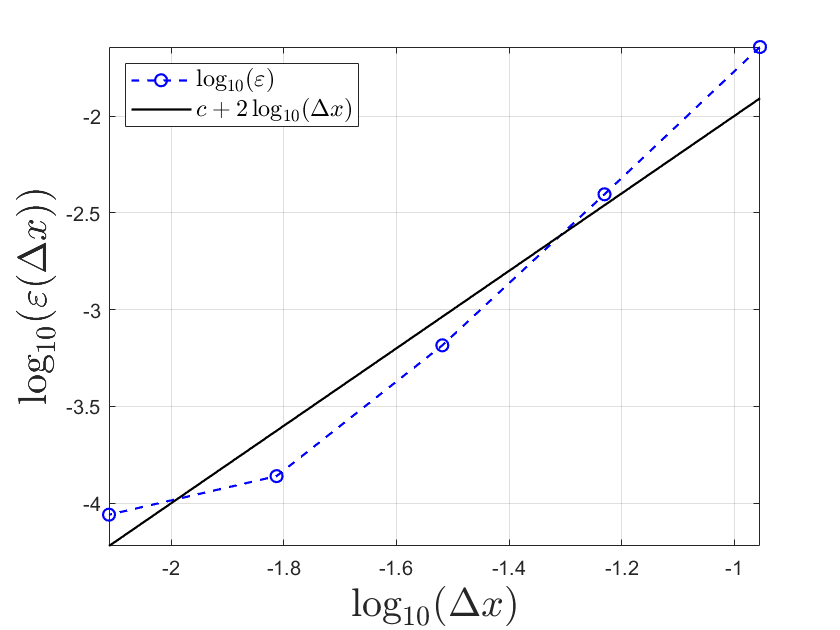
\includegraphics[scale = 0.3]{prob_1_2log_err.png}
            \end{center}
        \end{figure}
        \begin{figure}[H]
            \begin{center}
                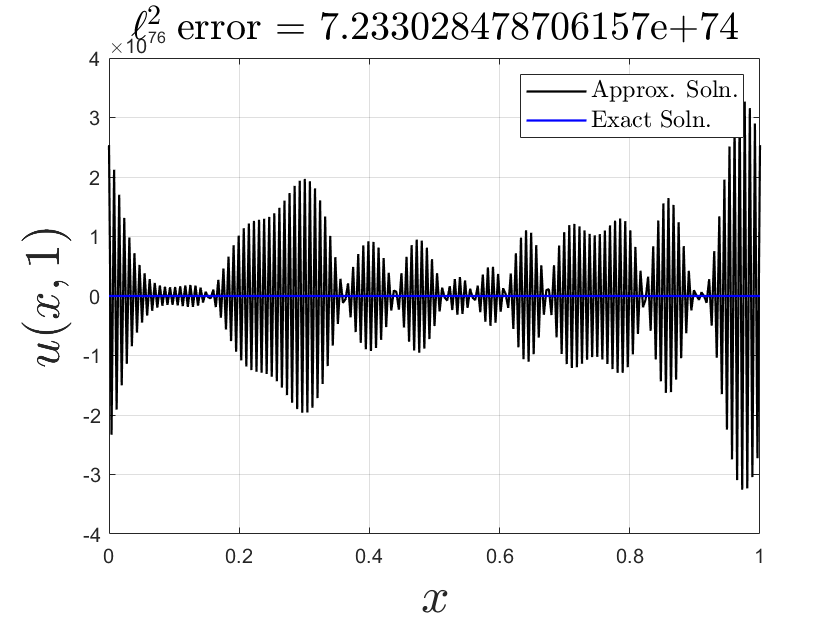
\includegraphics[scale = 0.3]{prob_1_2_nx_257.png}
            \end{center}
        \end{figure}
        
    \end{itemize}


    \pagebreak
    \item[\textbf{2}.] Consider a linear convection equation:
    \[\frac{\partial u}{\partial t} + c\frac{\partial u}{\partial x} = 0\]
    in which $c = 1$. The initial condition of $u$ is $u(x,0) = \exp{(-(x - 2)^2)}.$ The computational domain is $x \in [0,L]$, where $L = 20$. Use the (1) Upwind scheme, (2) Lax scheme, (3) Lax-Wendroff scheme, and (4) MacCormack scheme calculating $u(x,t)$ at $t = 10$. Set $\nu = \frac{c\Delta t}{\Delta x} = 0.5$.
    \newline\newline
    Objective: study the effects of $\Delta x$ on diffusion and dispersion error.
    \newline
    2.1 Take $\Delta x = 1.0$
    \newline
    2.2 Take $\Delta x = 0.5$
    \newline
    2.3 Take $\Delta x = 0.2$
    \newline
    2.4 Take $\Delta x = 0.1$
    \newline\newline
    Plot the exact solution and the results from various schemes for each $\Delta x$. Observe how the diffusion and dispersion error changes with $\Delta x$. This problem shows us why higher spatial resolution improves the accuracy. In linear advection equation, the MacCormack scheme is equivalent to the Lax-Wendroff scheme.
    \newline\newline
    To get better understanding of the various schemes, recall the modified equation.
    \newline\newline
    Modified equation of the upwind scheme:
    \[\frac{\partial u}{\partial t} + a\frac{\partial u}{\partial x} = \frac{a\Delta x}{2}(1 - \nu)\frac{\partial^2u}{\partial x^2} + \frac{a(\Delta x)^2}{6}(3\nu - 2\nu^2 - 1)\frac{\partial^3u}{\partial x^3} + \mathcal{O}((\Delta t)^3, (\Delta t)^2\Delta x, \Delta t(\Delta x)^2, (\Delta x)^3)\]
    Modified equation of the Lax scheme:
    \[\frac{\partial u}{\partial t} + a\frac{\partial u}{\partial x} = \frac{a\Delta x}{2}\left(\frac{1}{\nu} - \nu\right)\frac{\partial^2u}{\partial x^2} + \frac{a(\Delta x)^2}{3}(1 - \nu^2)\frac{\partial^3u}{\partial x^3} + \cdots\]
    Modified equation of the Lax-Wendroff scheme:
    \[\frac{\partial u}{\partial t} + a\frac{\partial u}{\partial x} = -\frac{a(\Delta x)^2}{6}(1 - \nu^2)\frac{\partial^3u}{\partial x^3} - \frac{a(\Delta x)^3}{8}\nu(1 - \nu^2)\frac{\partial^4u}{\partial x^4} + \cdots\]
    \textit{Soln.}
    \begin{itemize}
        \item[(1)] Upwind scheme:
        \newline\newline
        Upon implementing the upwind scheme for the 1D linear advection equation, we find the following plots for the approximate and exact solutions for varying values of $\Delta x$:
        \begin{figure}[H]
        \begin{center}
            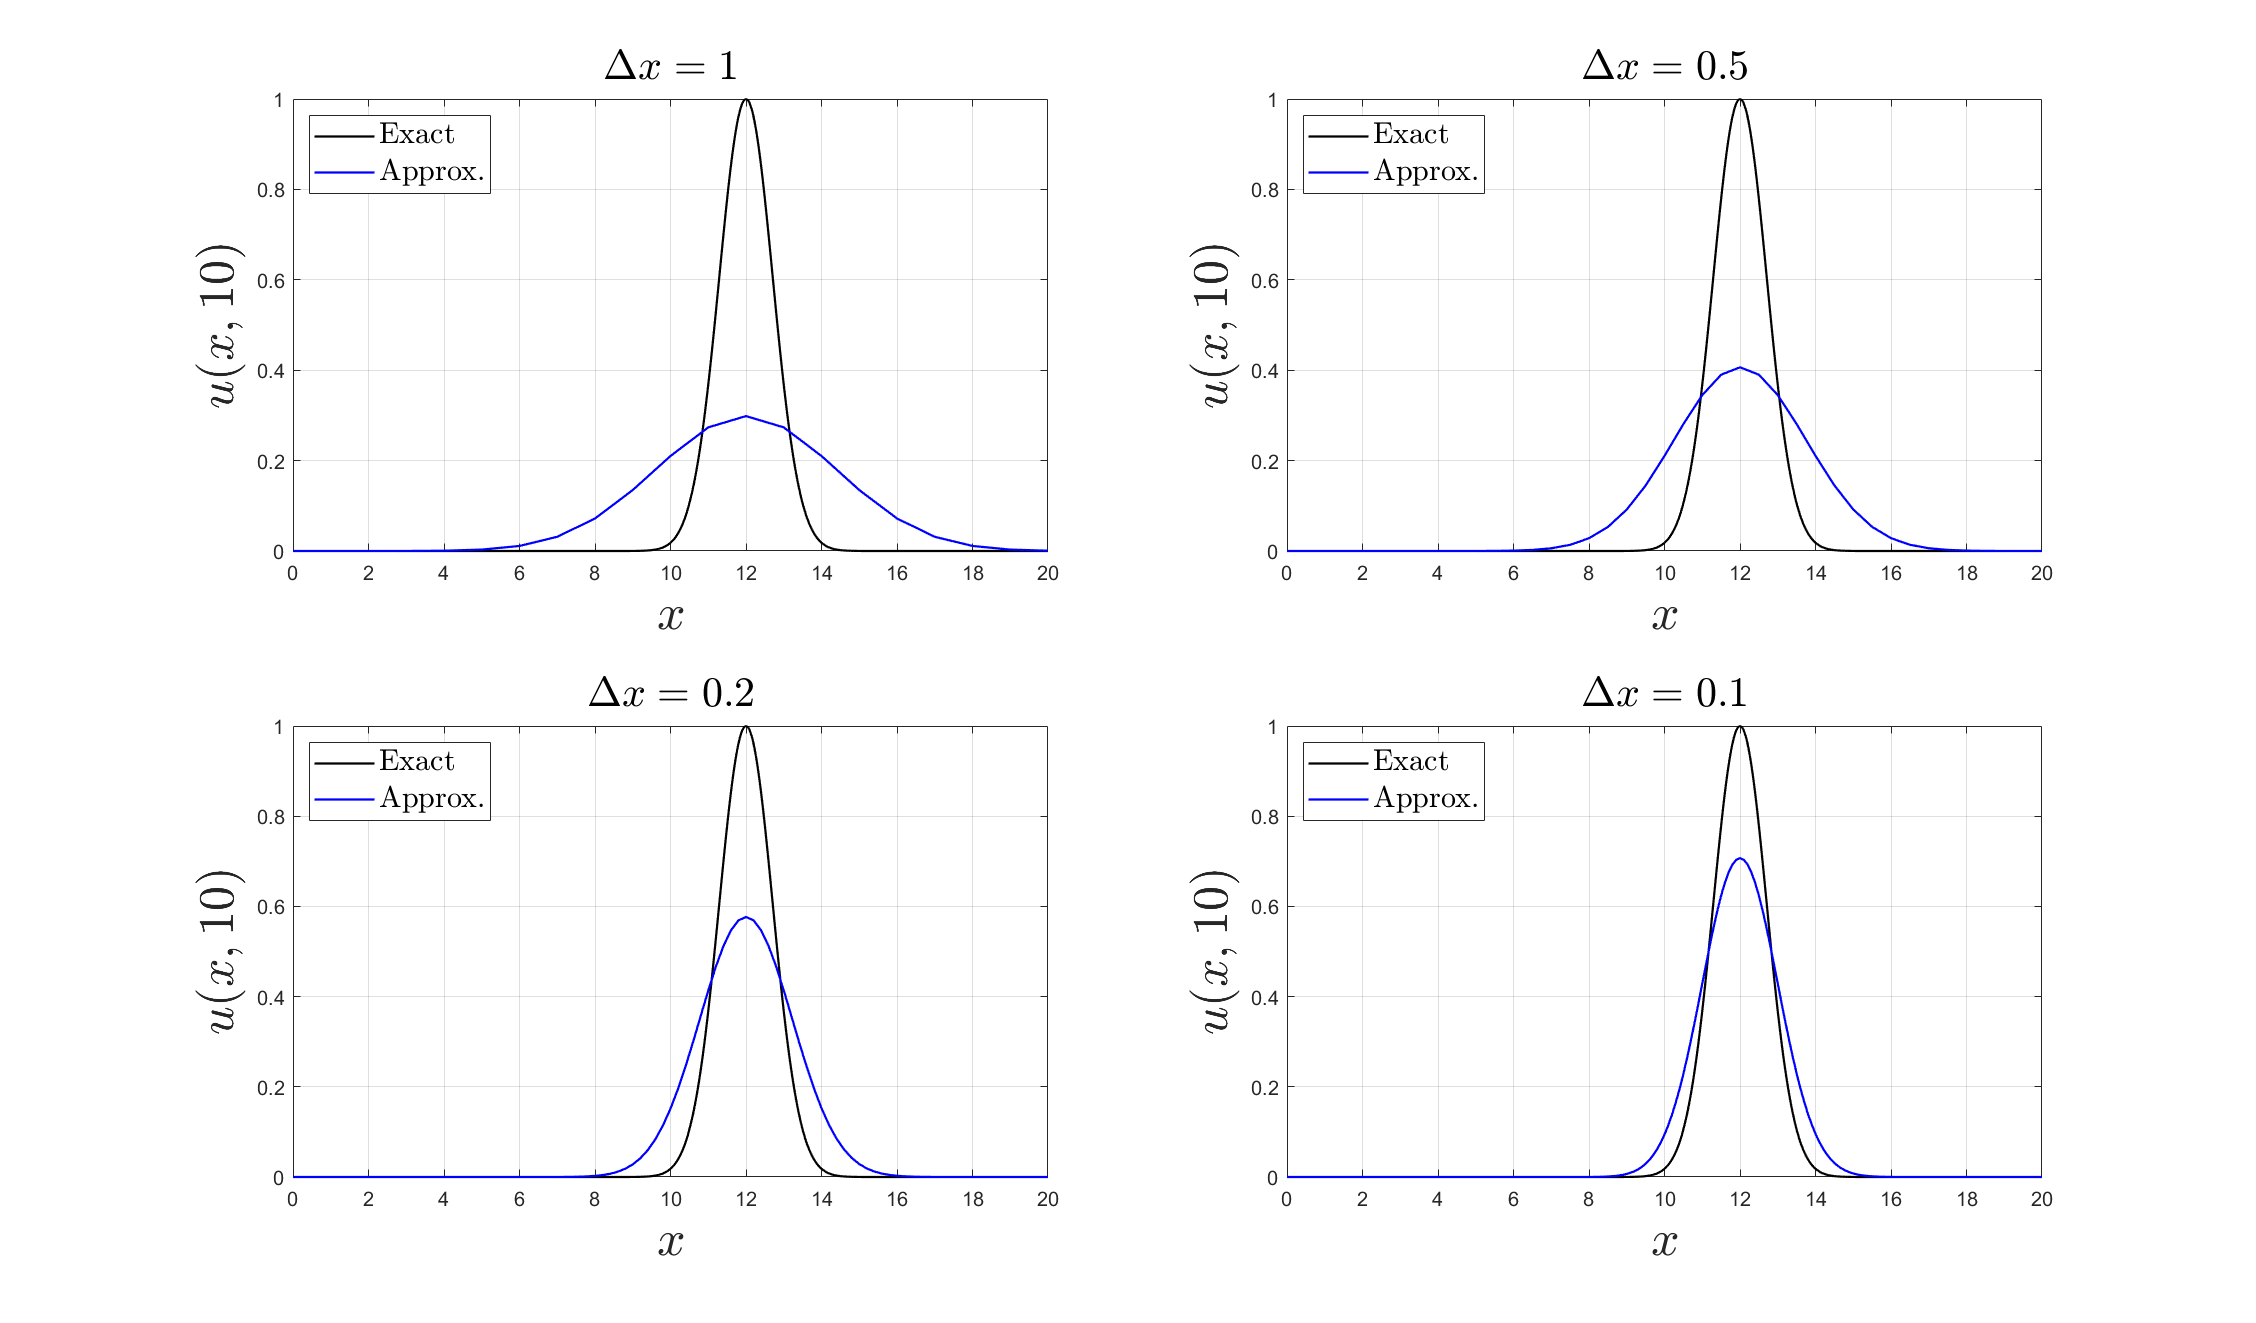
\includegraphics[scale = 0.25]{prob_2_upwind_subplots.png}
            \caption{Numerical solutions to the linear advection equation with given initial guess and varying values of $\Delta x$.}
        \end{center}
        \end{figure}


        \item[(2)] Lax scheme:
        \newline\newline
        \begin{figure}[H]
        \begin{center}
            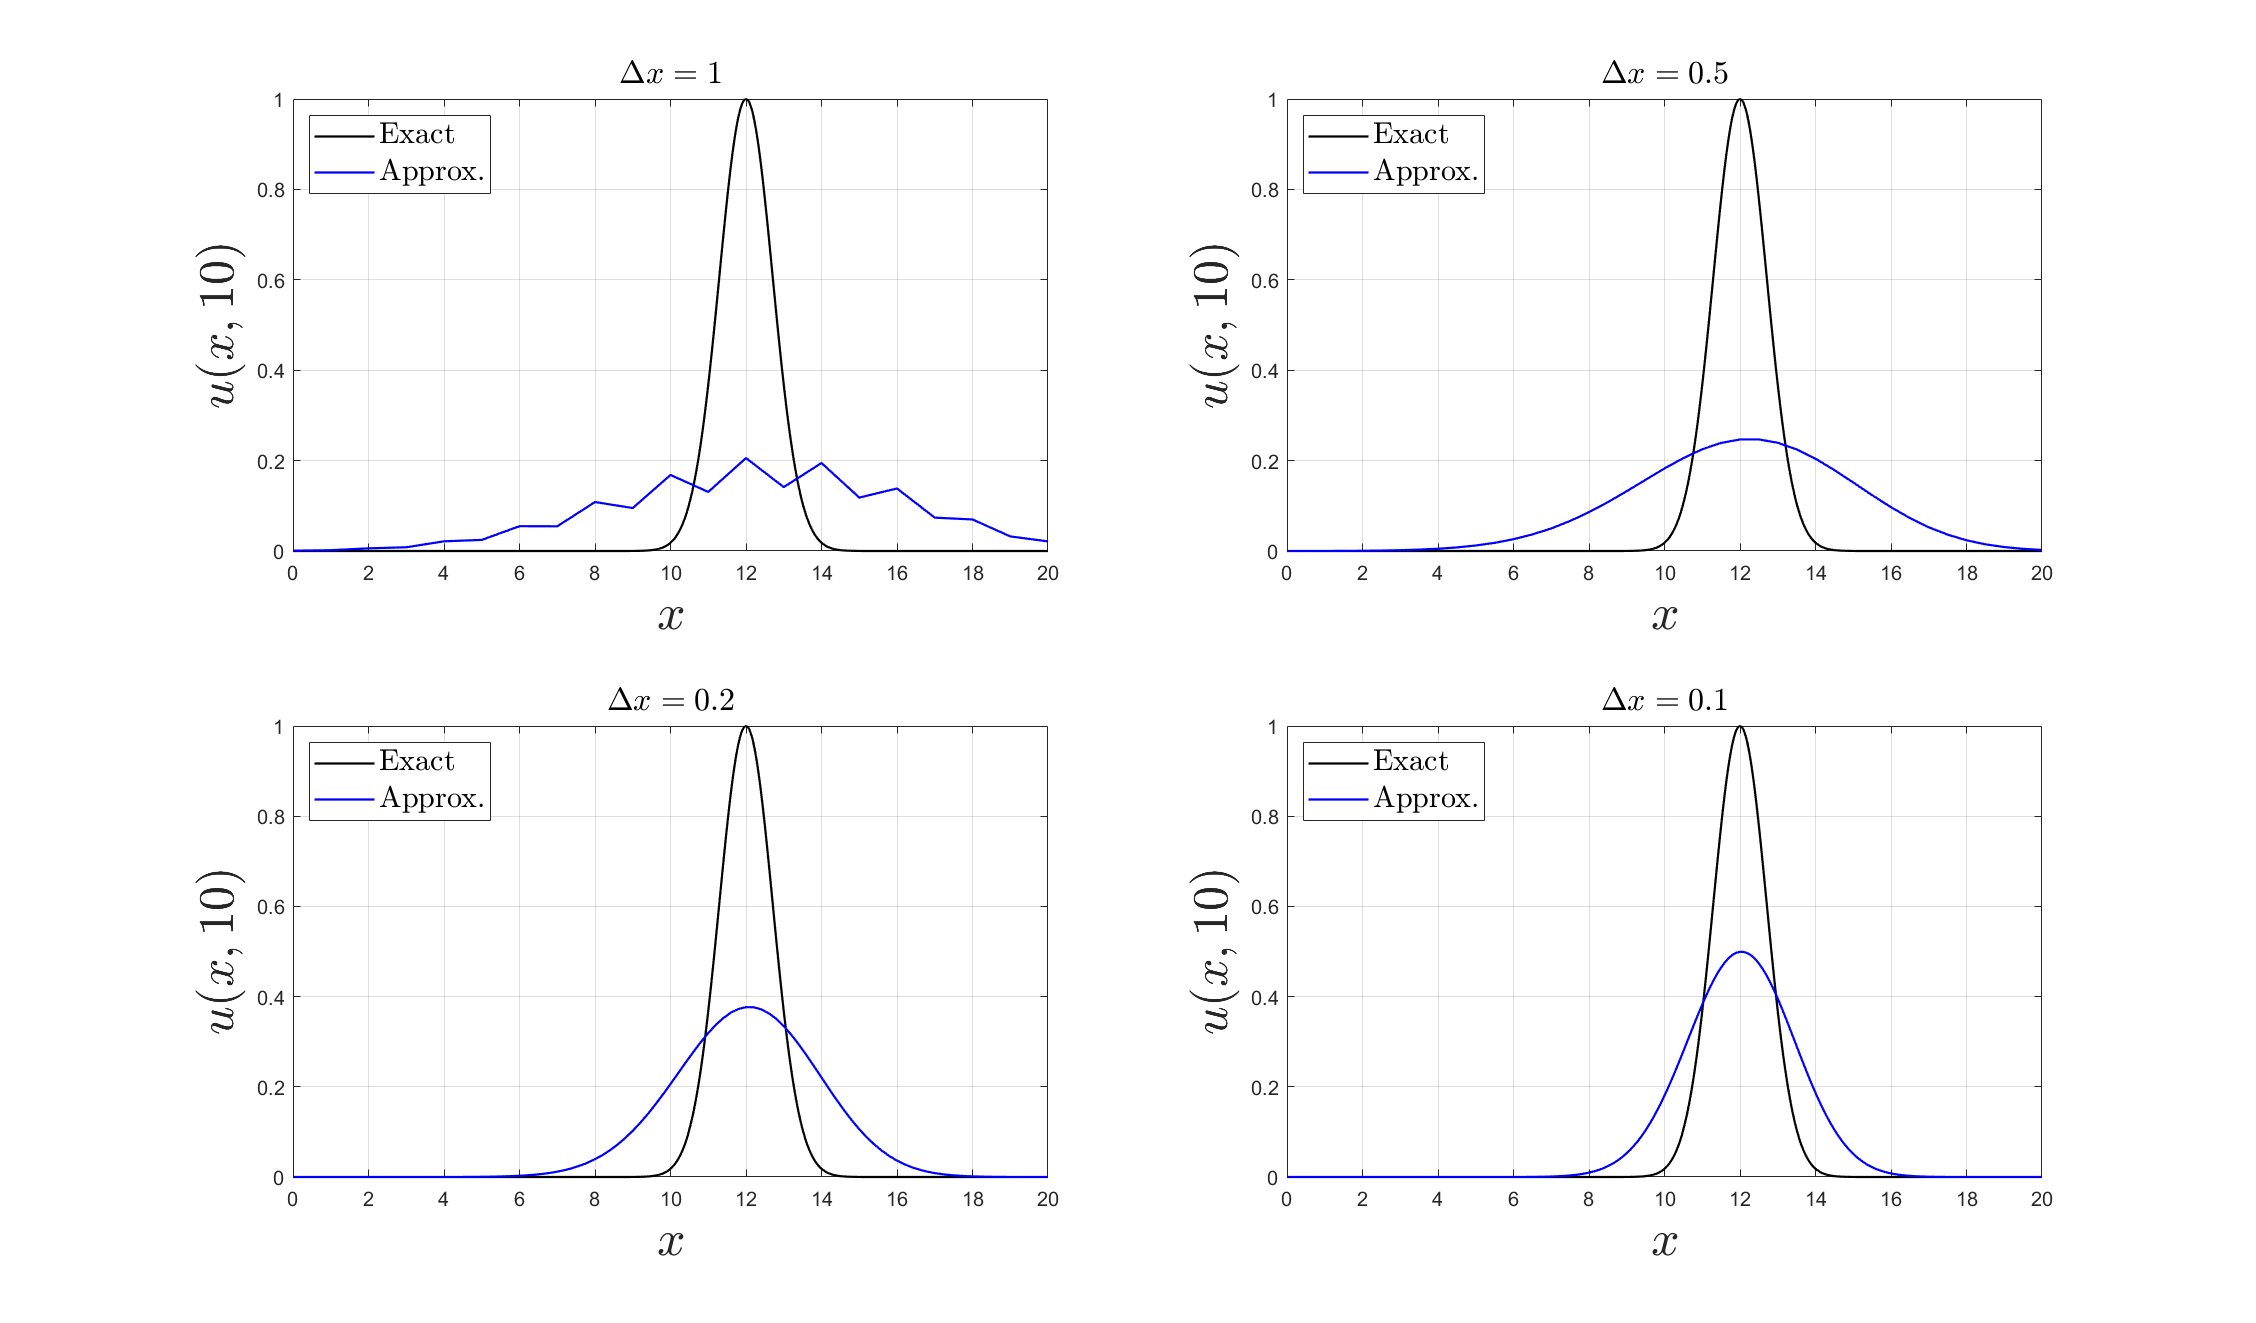
\includegraphics[scale = 0.25]{prob_2_lax_subplots.png}
        \end{center}
        \end{figure}

        \item[(3)] Lax-Wendroff scheme:
        \newline\newline
        \begin{figure}[H]
            \begin{center}
            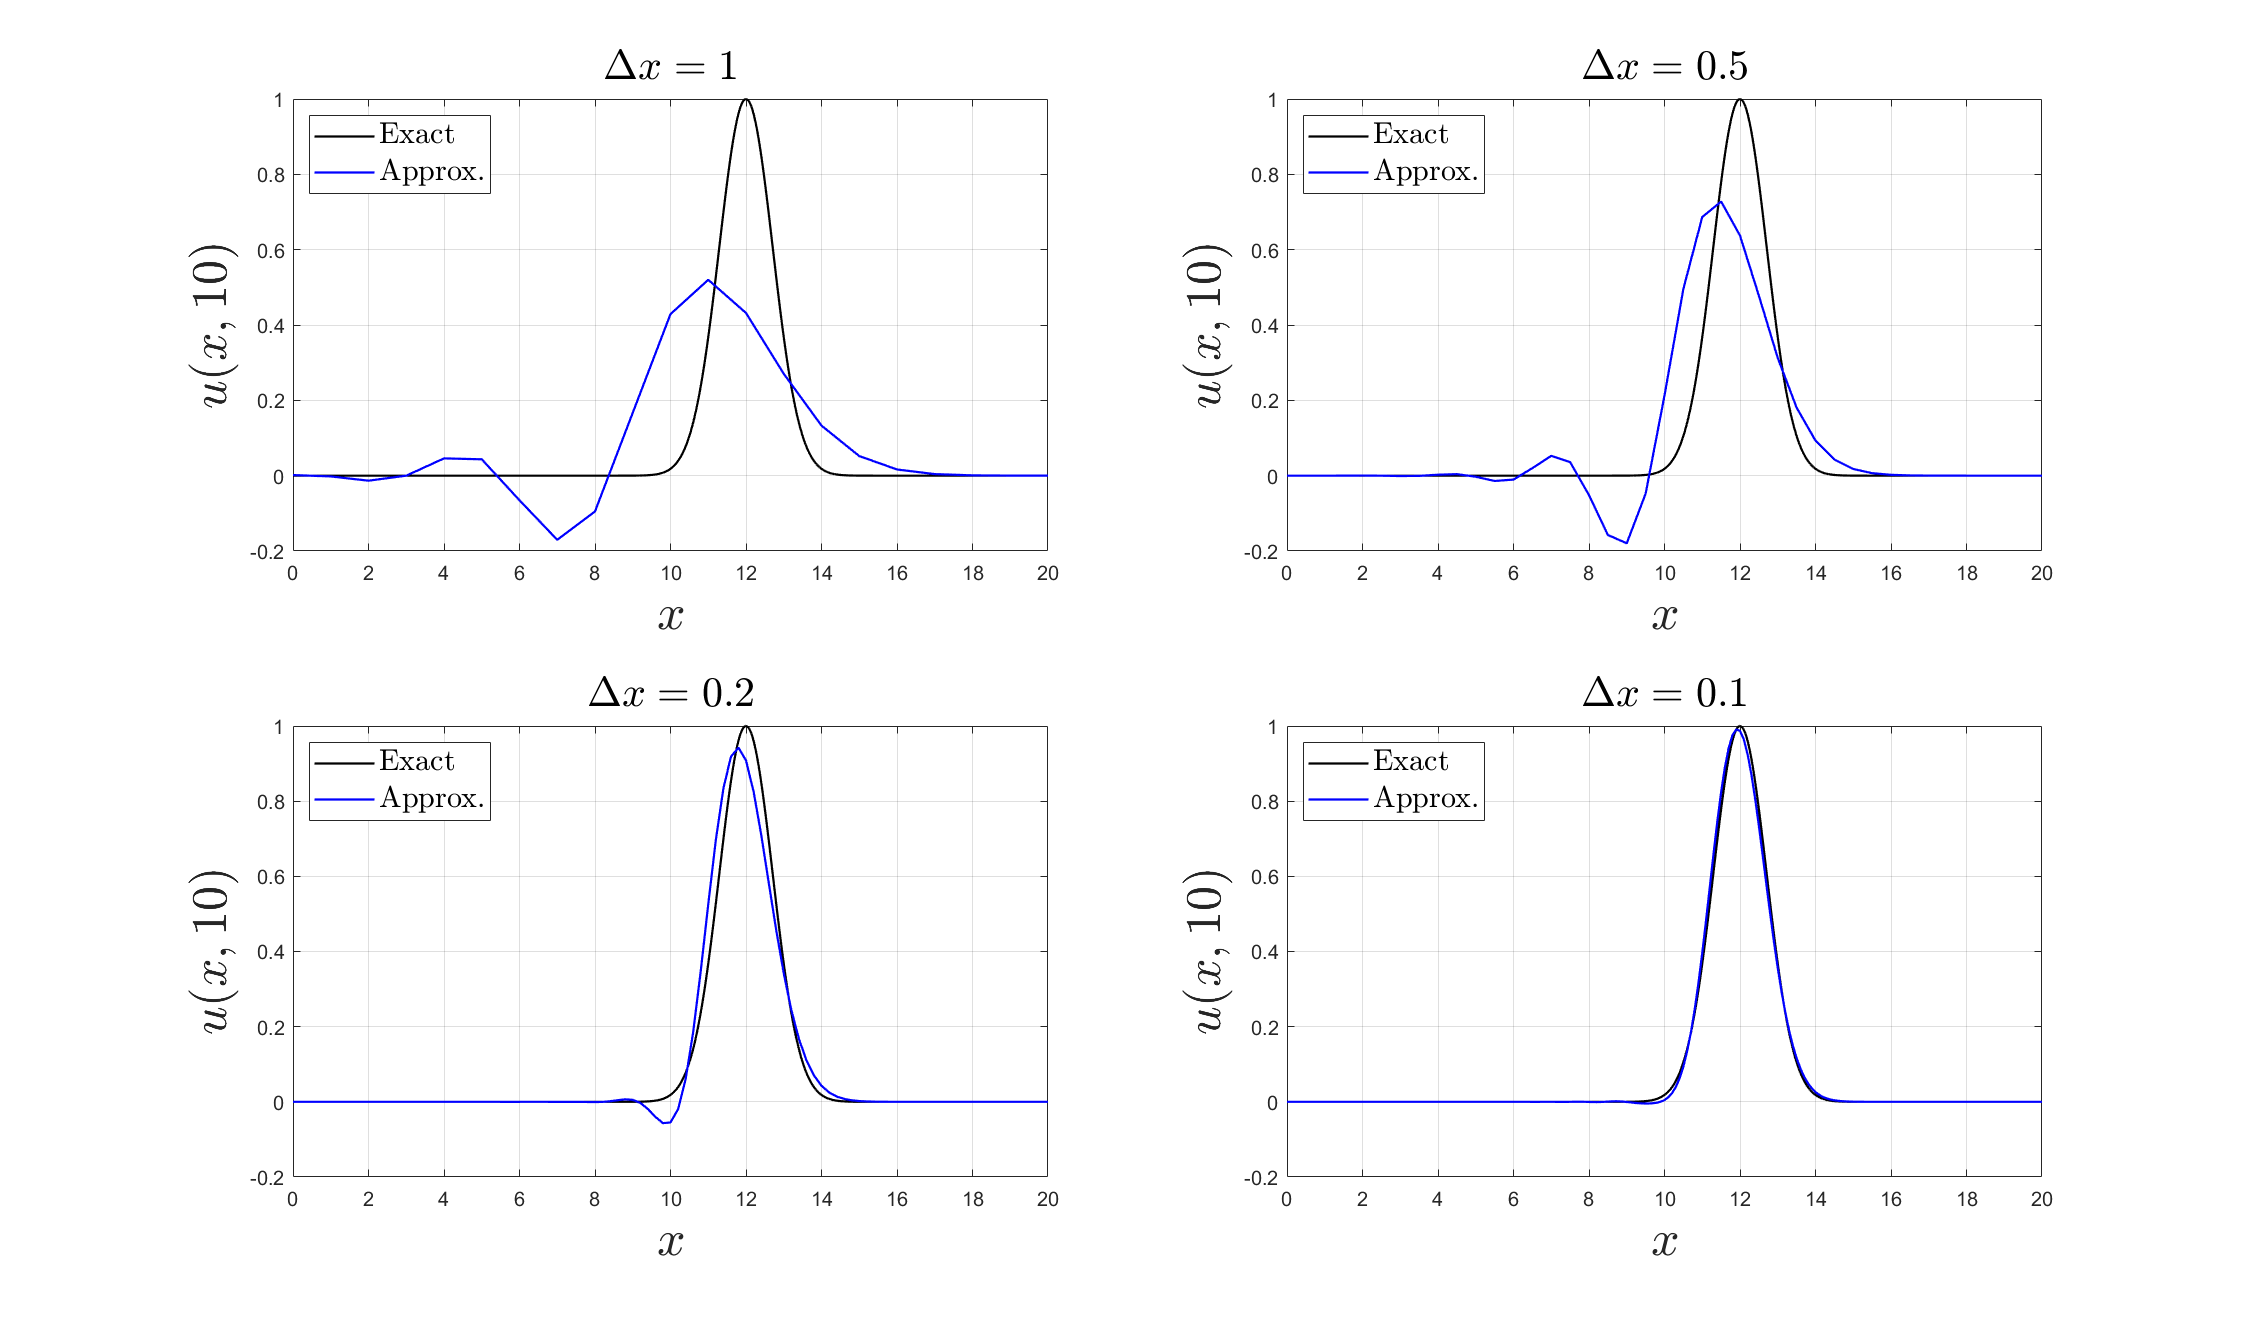
\includegraphics[scale = 0.25]{prob_2_laxwendroff_subplots.png}
            \end{center}
        \end{figure}

        \item[(4)] MacCormack scheme:
        \newline\newline
        \begin{figure}[H]
        \begin{center}
            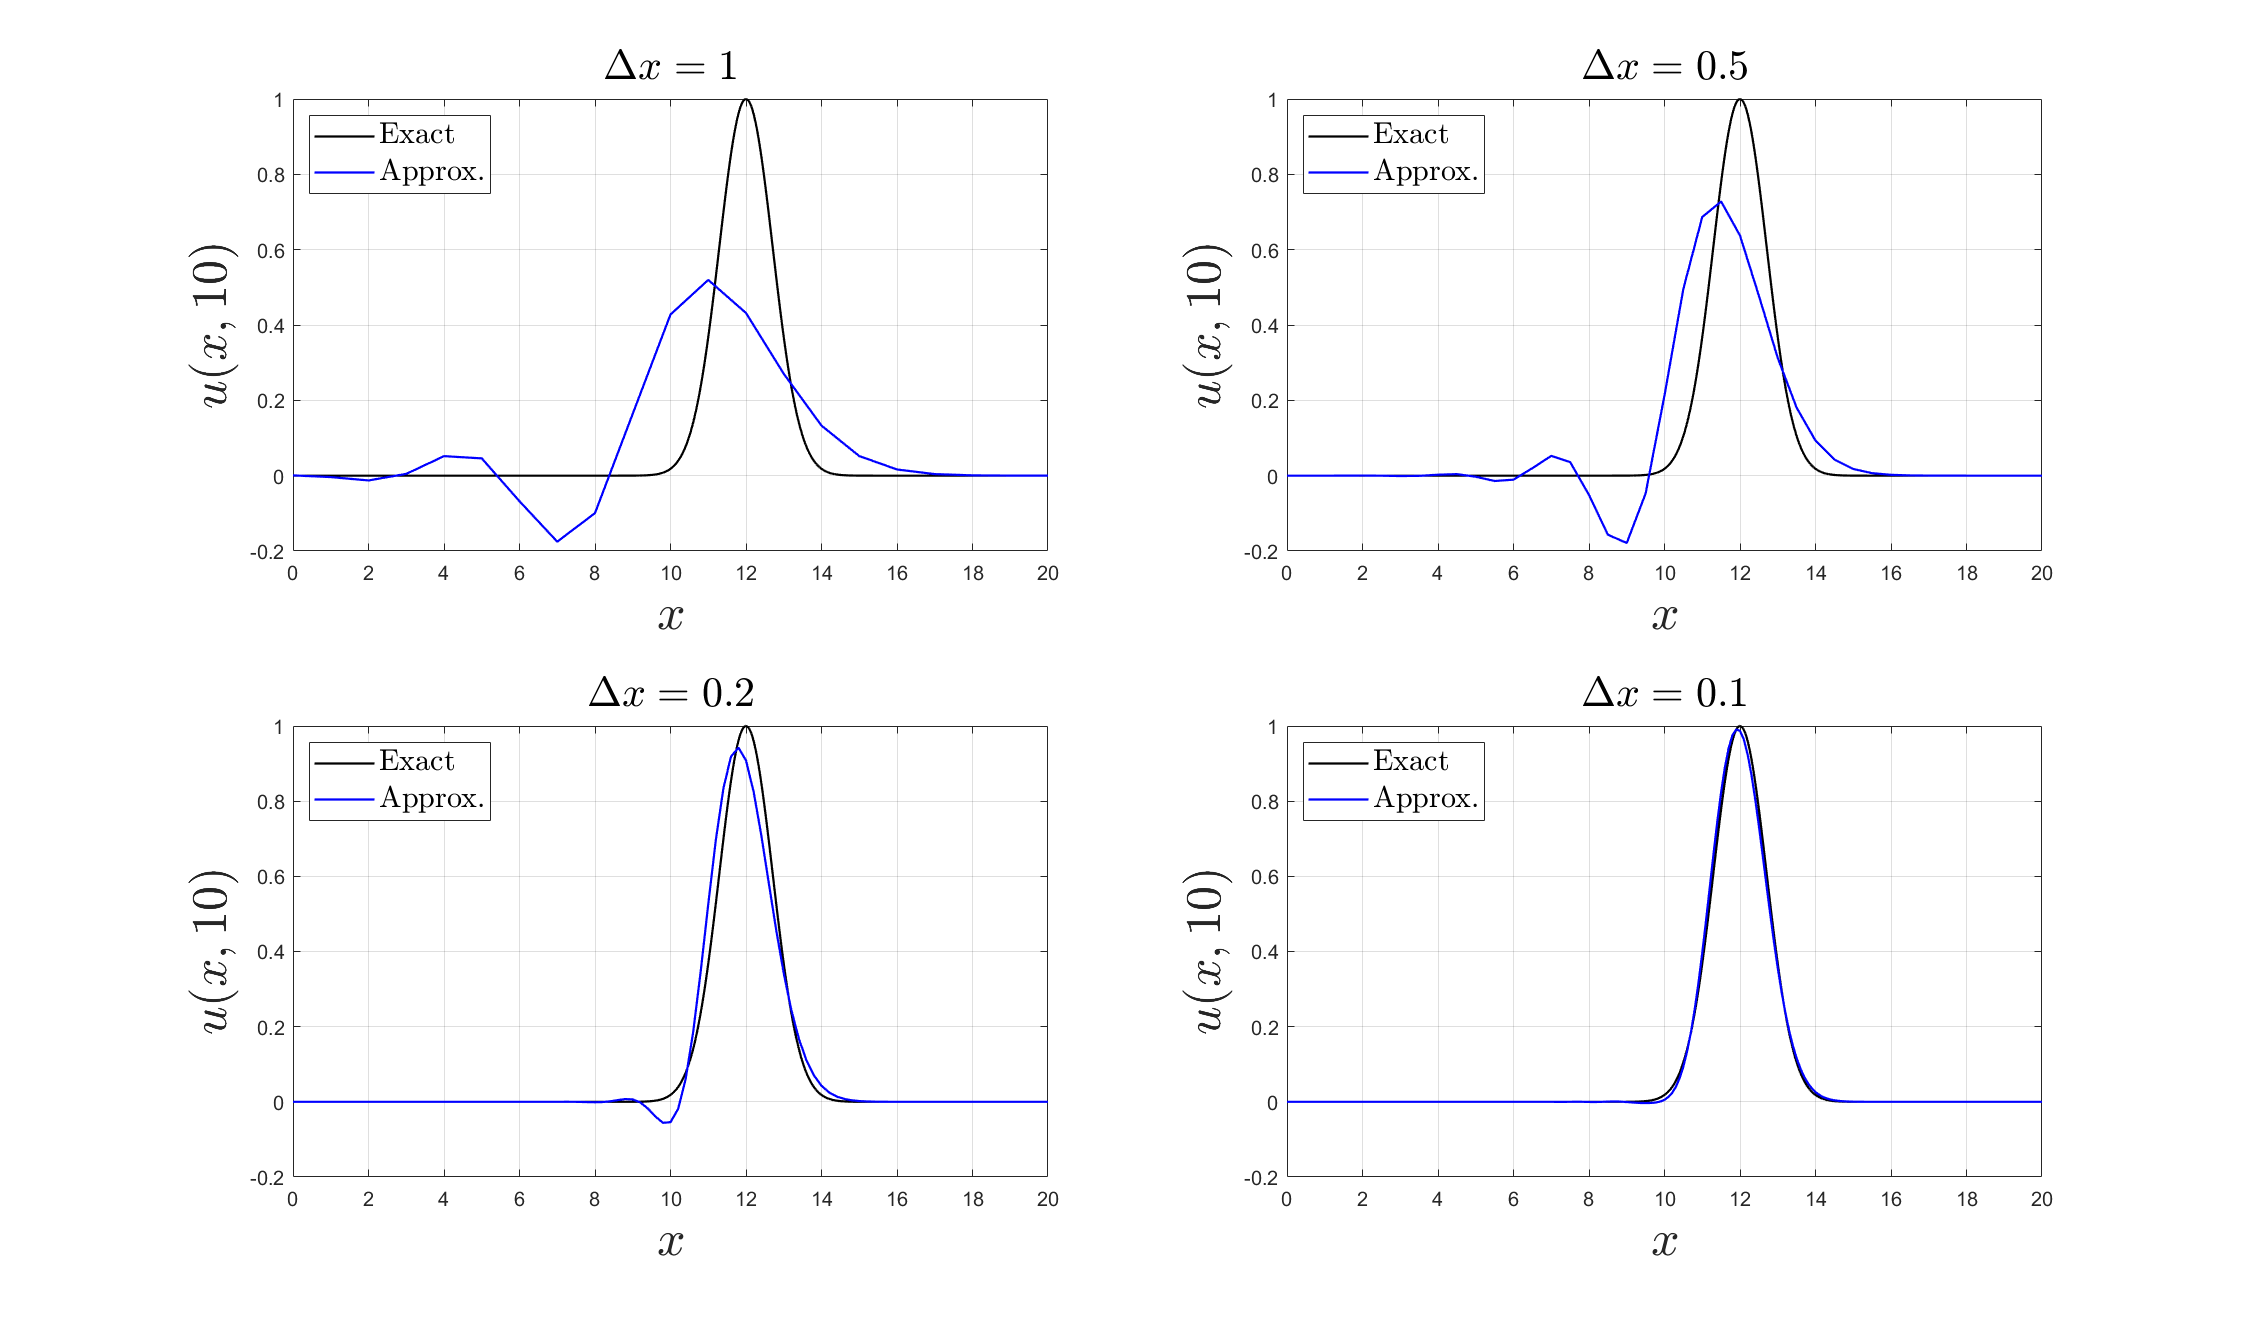
\includegraphics[scale = 0.25]{prob_2_maccormack_subplots.png}
        \end{center}
        \end{figure}
        
    \end{itemize}



    \pagebreak
    \item[\textbf{3}.] Consider a linear convection equation:
    \[\frac{\partial u}{\partial t} + c\frac{\partial u}{\partial x} = 0\]
    in which $c = 1$. The initial condition of $u$ is
    \[u(x,0) = \begin{cases}
        1, & x \leq 0\\
        0, & x > 0
    \end{cases}\]
    The computational domain is $x \in [0,10]$, use the (1) Upwind scheme, (2) Lax scheme, (3) Lax-Wendroff scheme, and (4) MacCormack scheme calculating $u(x,t)$ at $t = 5$. Set $\Delta x = 0.1$.
    \newline\newline
    3.1 Take $\nu = \frac{c\Delta t}{\Delta x} = 1.0$
    \newline
    3.2 Take $\nu = \frac{c\Delta t}{\Delta x} = 0.75$
    \newline
    3.3 Take $\nu = \frac{c\Delta t}{\Delta x} = 0.25$.
    \newline\newline
    Plot the exact solution and the results of the four schemes all together, for each $\nu$. Does smaller $\Delta t$ always give better results? Why Lax scheme is more diffusive than the upwind scheme? Why the dispersive error is gone when $\nu = 1.0$?
    \newline\newline
    \textit{Soln.}
    \begin{itemize}
        \item[(1)] Upwind scheme:
        \newline\newline
        \begin{figure}[H]
            \begin{center}
                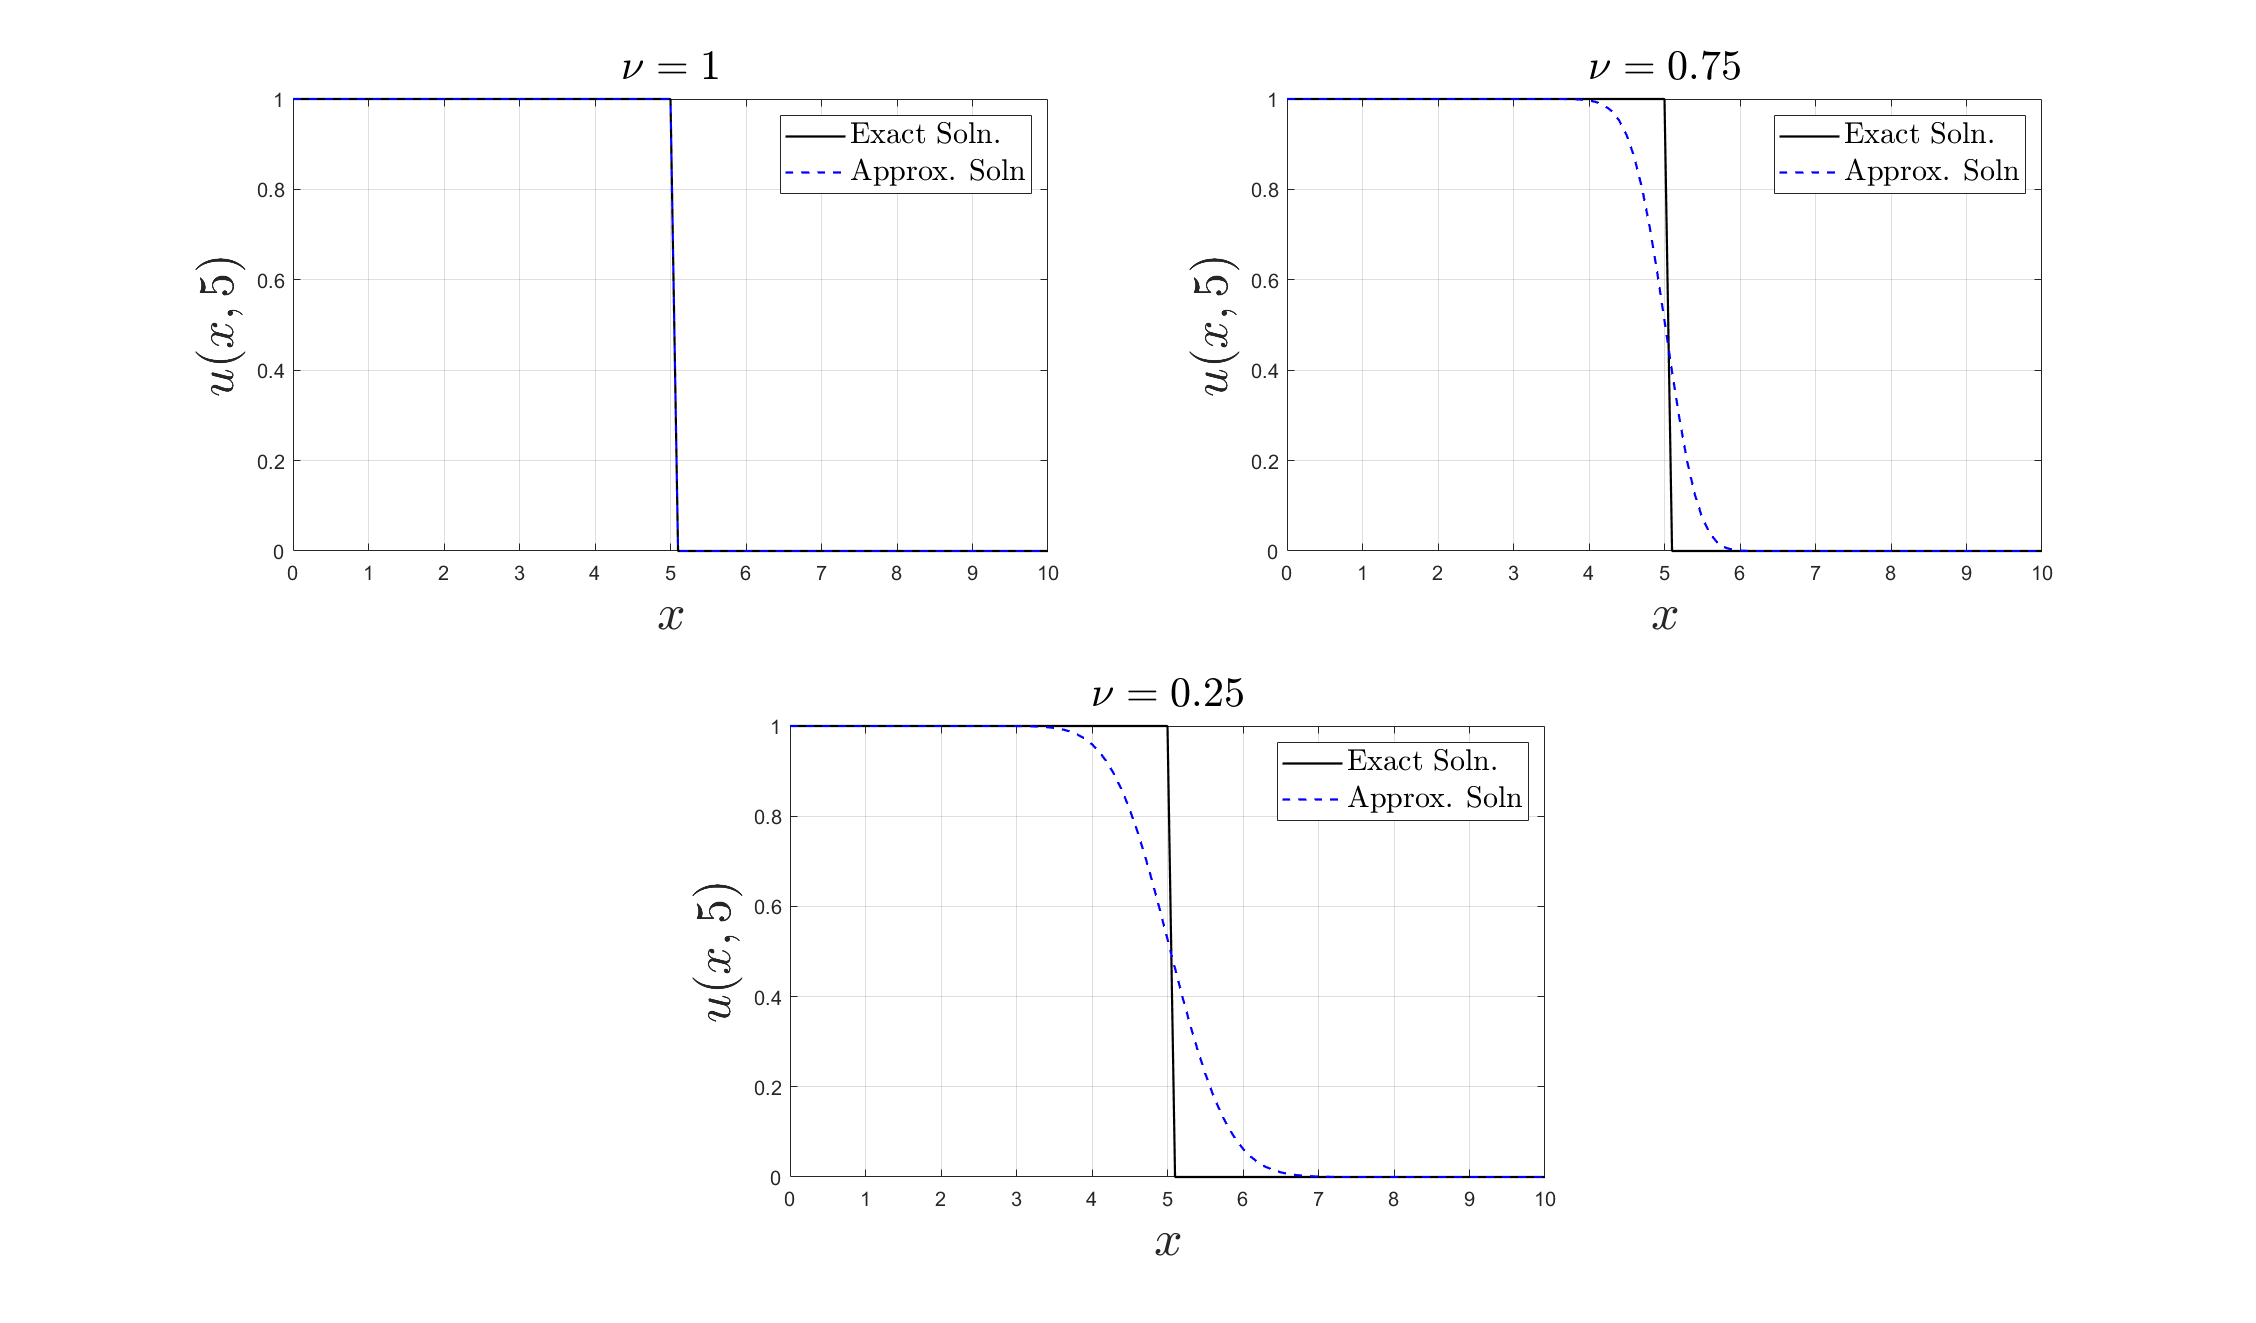
\includegraphics[scale = 0.25]{prob_3_upwind_subplots.png}
            \end{center}
        \end{figure}


        \item[(2)] Lax scheme:
        \newline\newline
        \begin{figure}[H]
            \begin{center}
                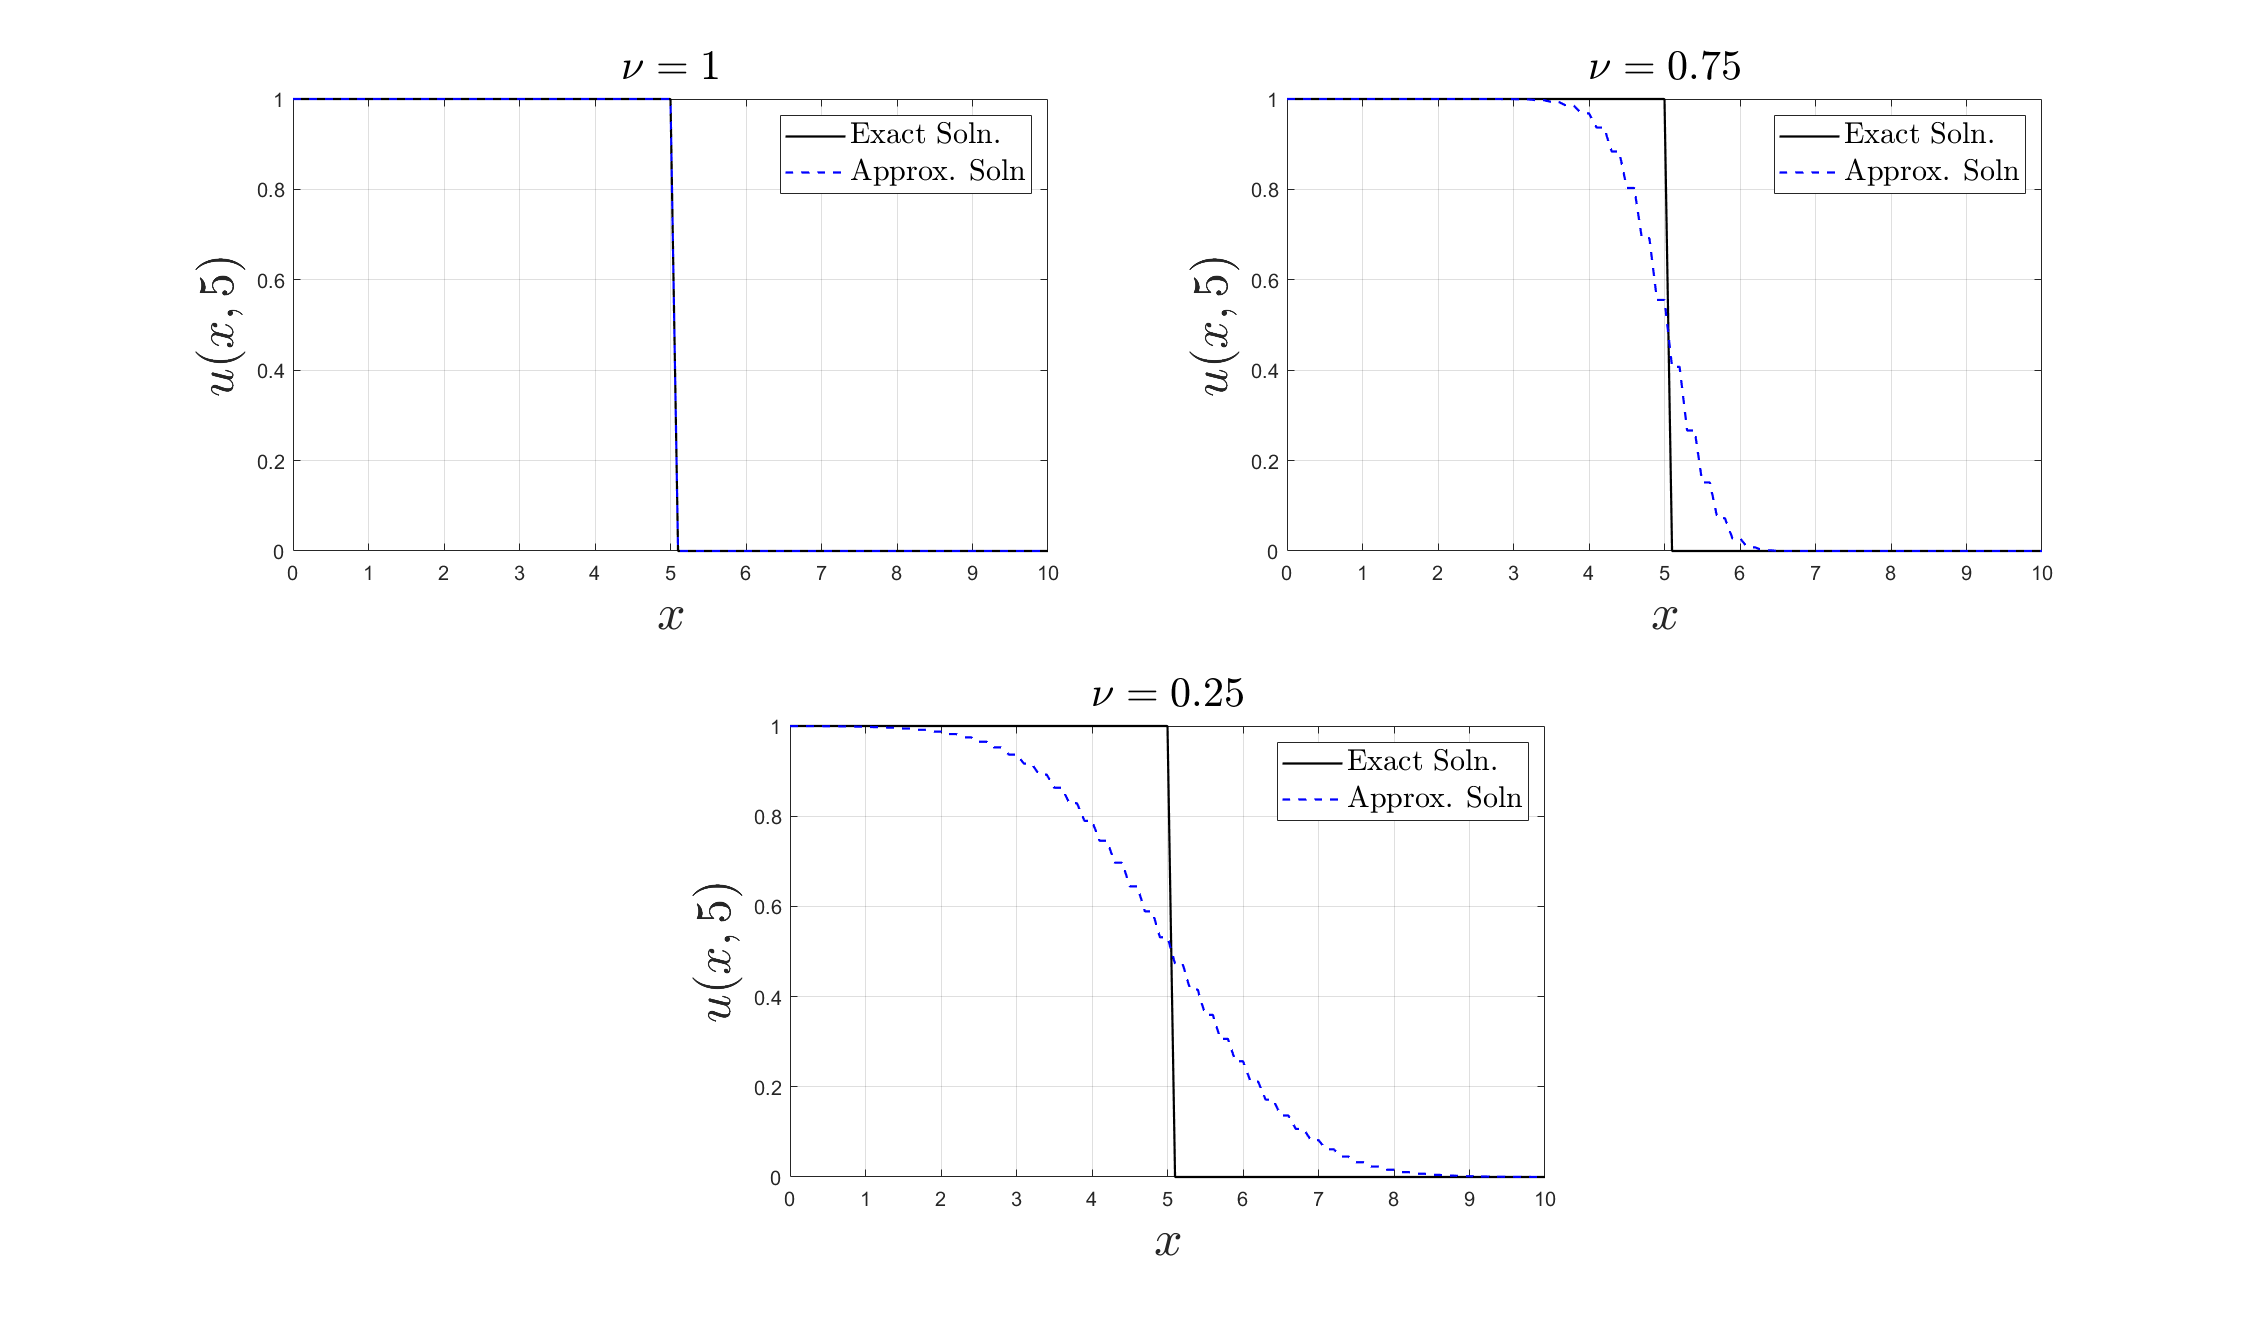
\includegraphics[scale = 0.25]{prob_3_lax_subplots.png}
            \end{center}
        \end{figure}

        \item[(3)] Lax-Wendroff scheme:
        \newline\newline
        \begin{figure}[H]
            \begin{center}
                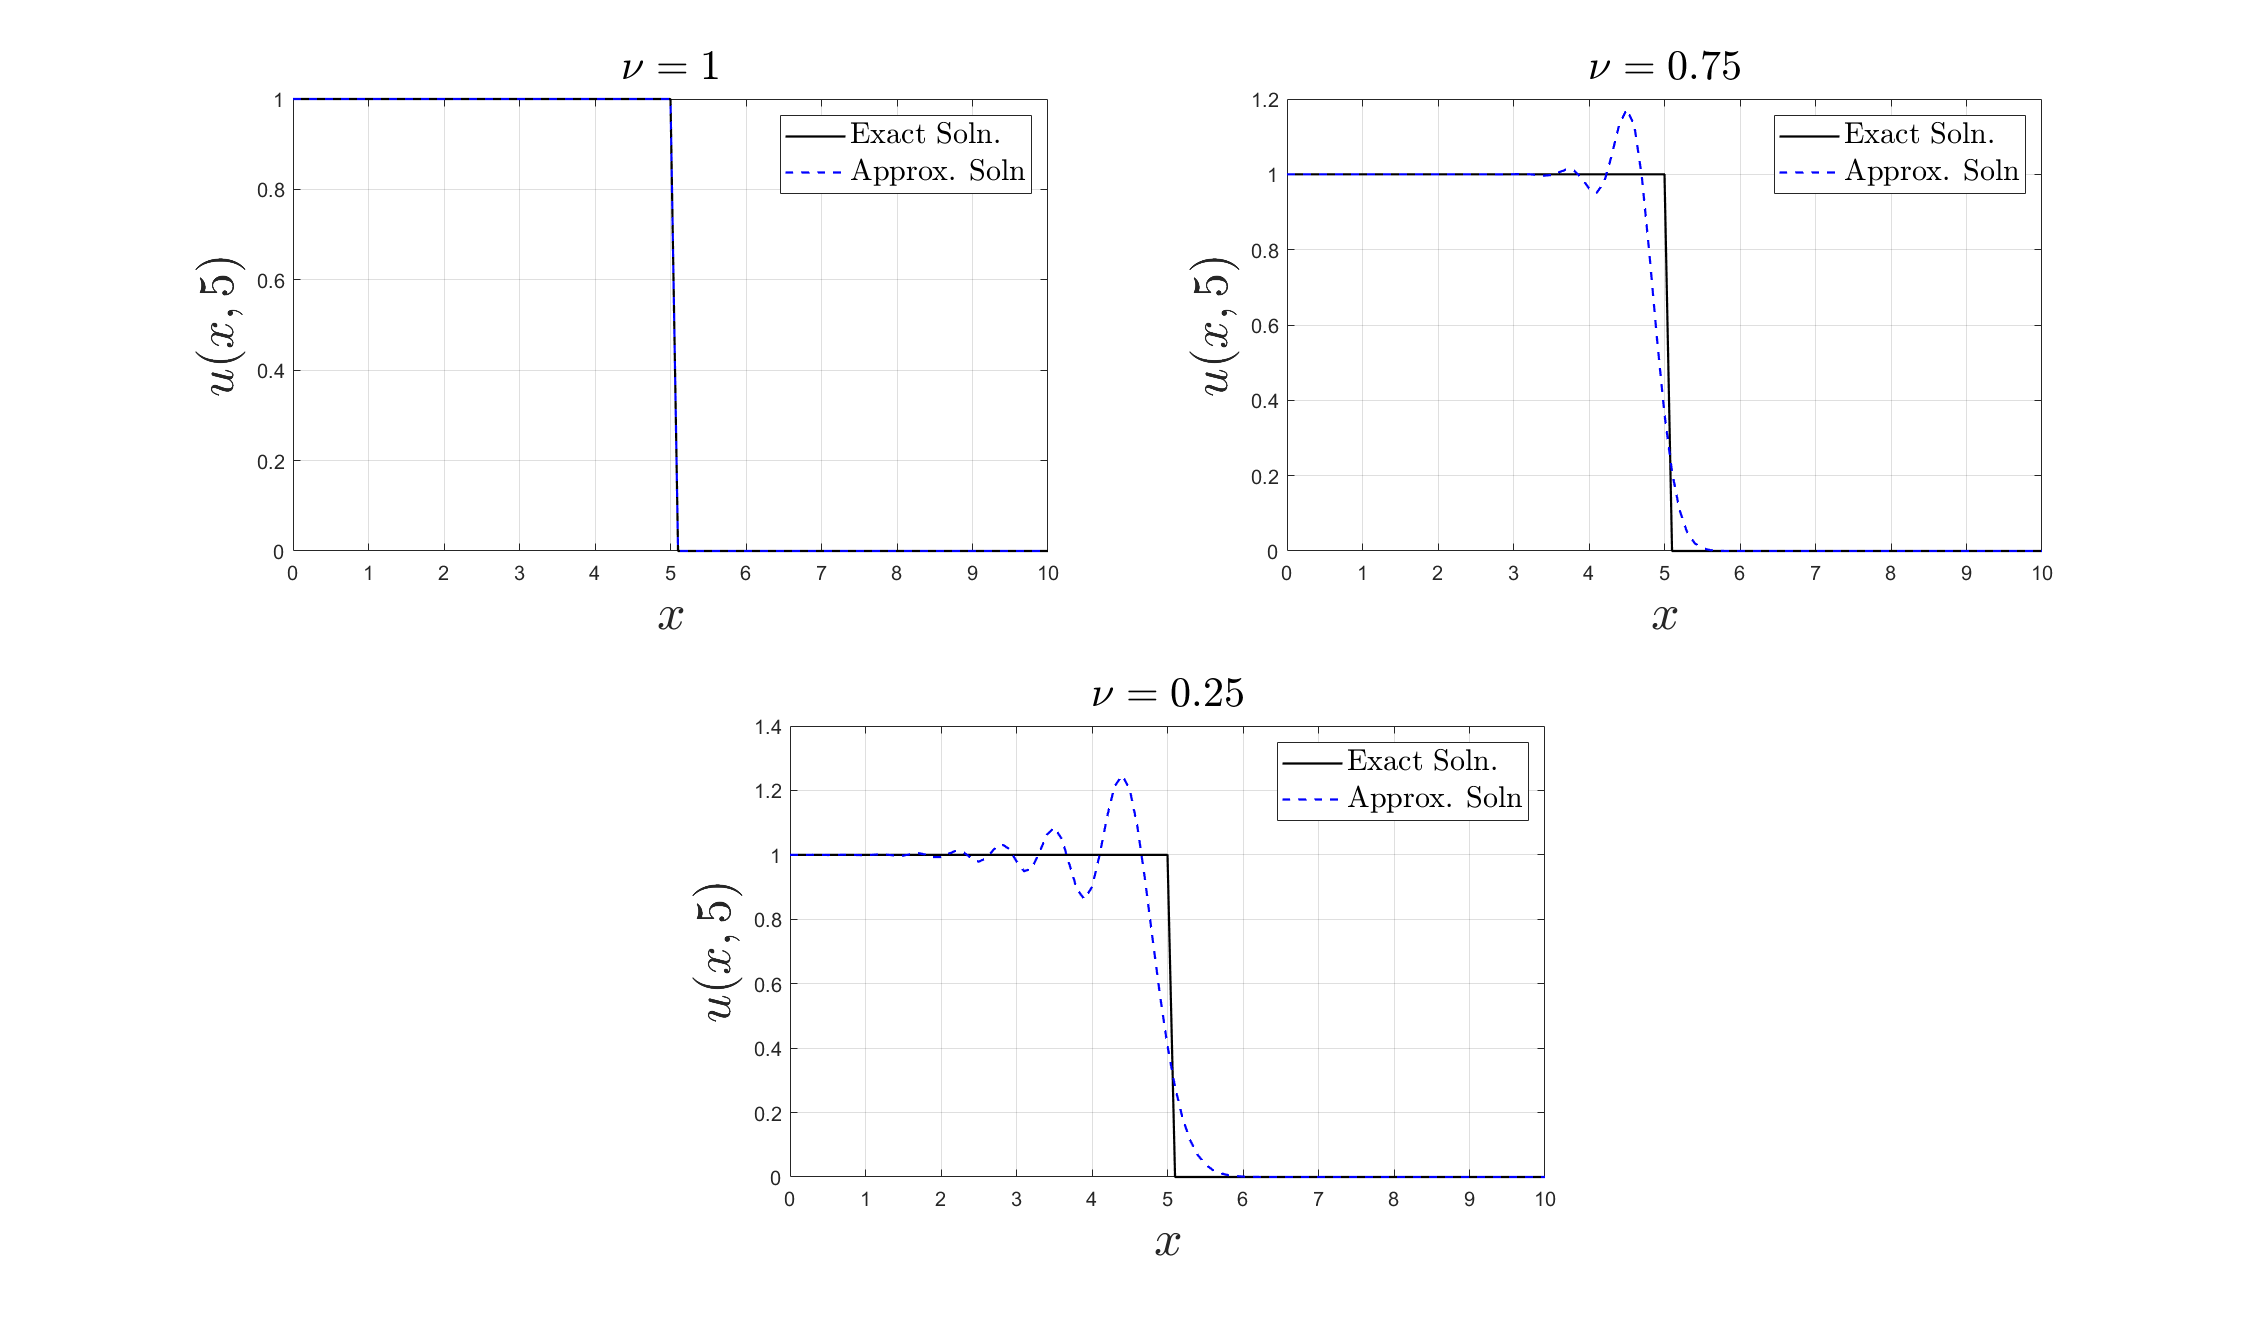
\includegraphics[scale = 0.25]{prob_3_laxwendroff_subplots.png}
            \end{center}
        \end{figure}


        \item[(4)] MacCormack scheme:
        \newline\newline
        \begin{figure}[H]
            \begin{center}
                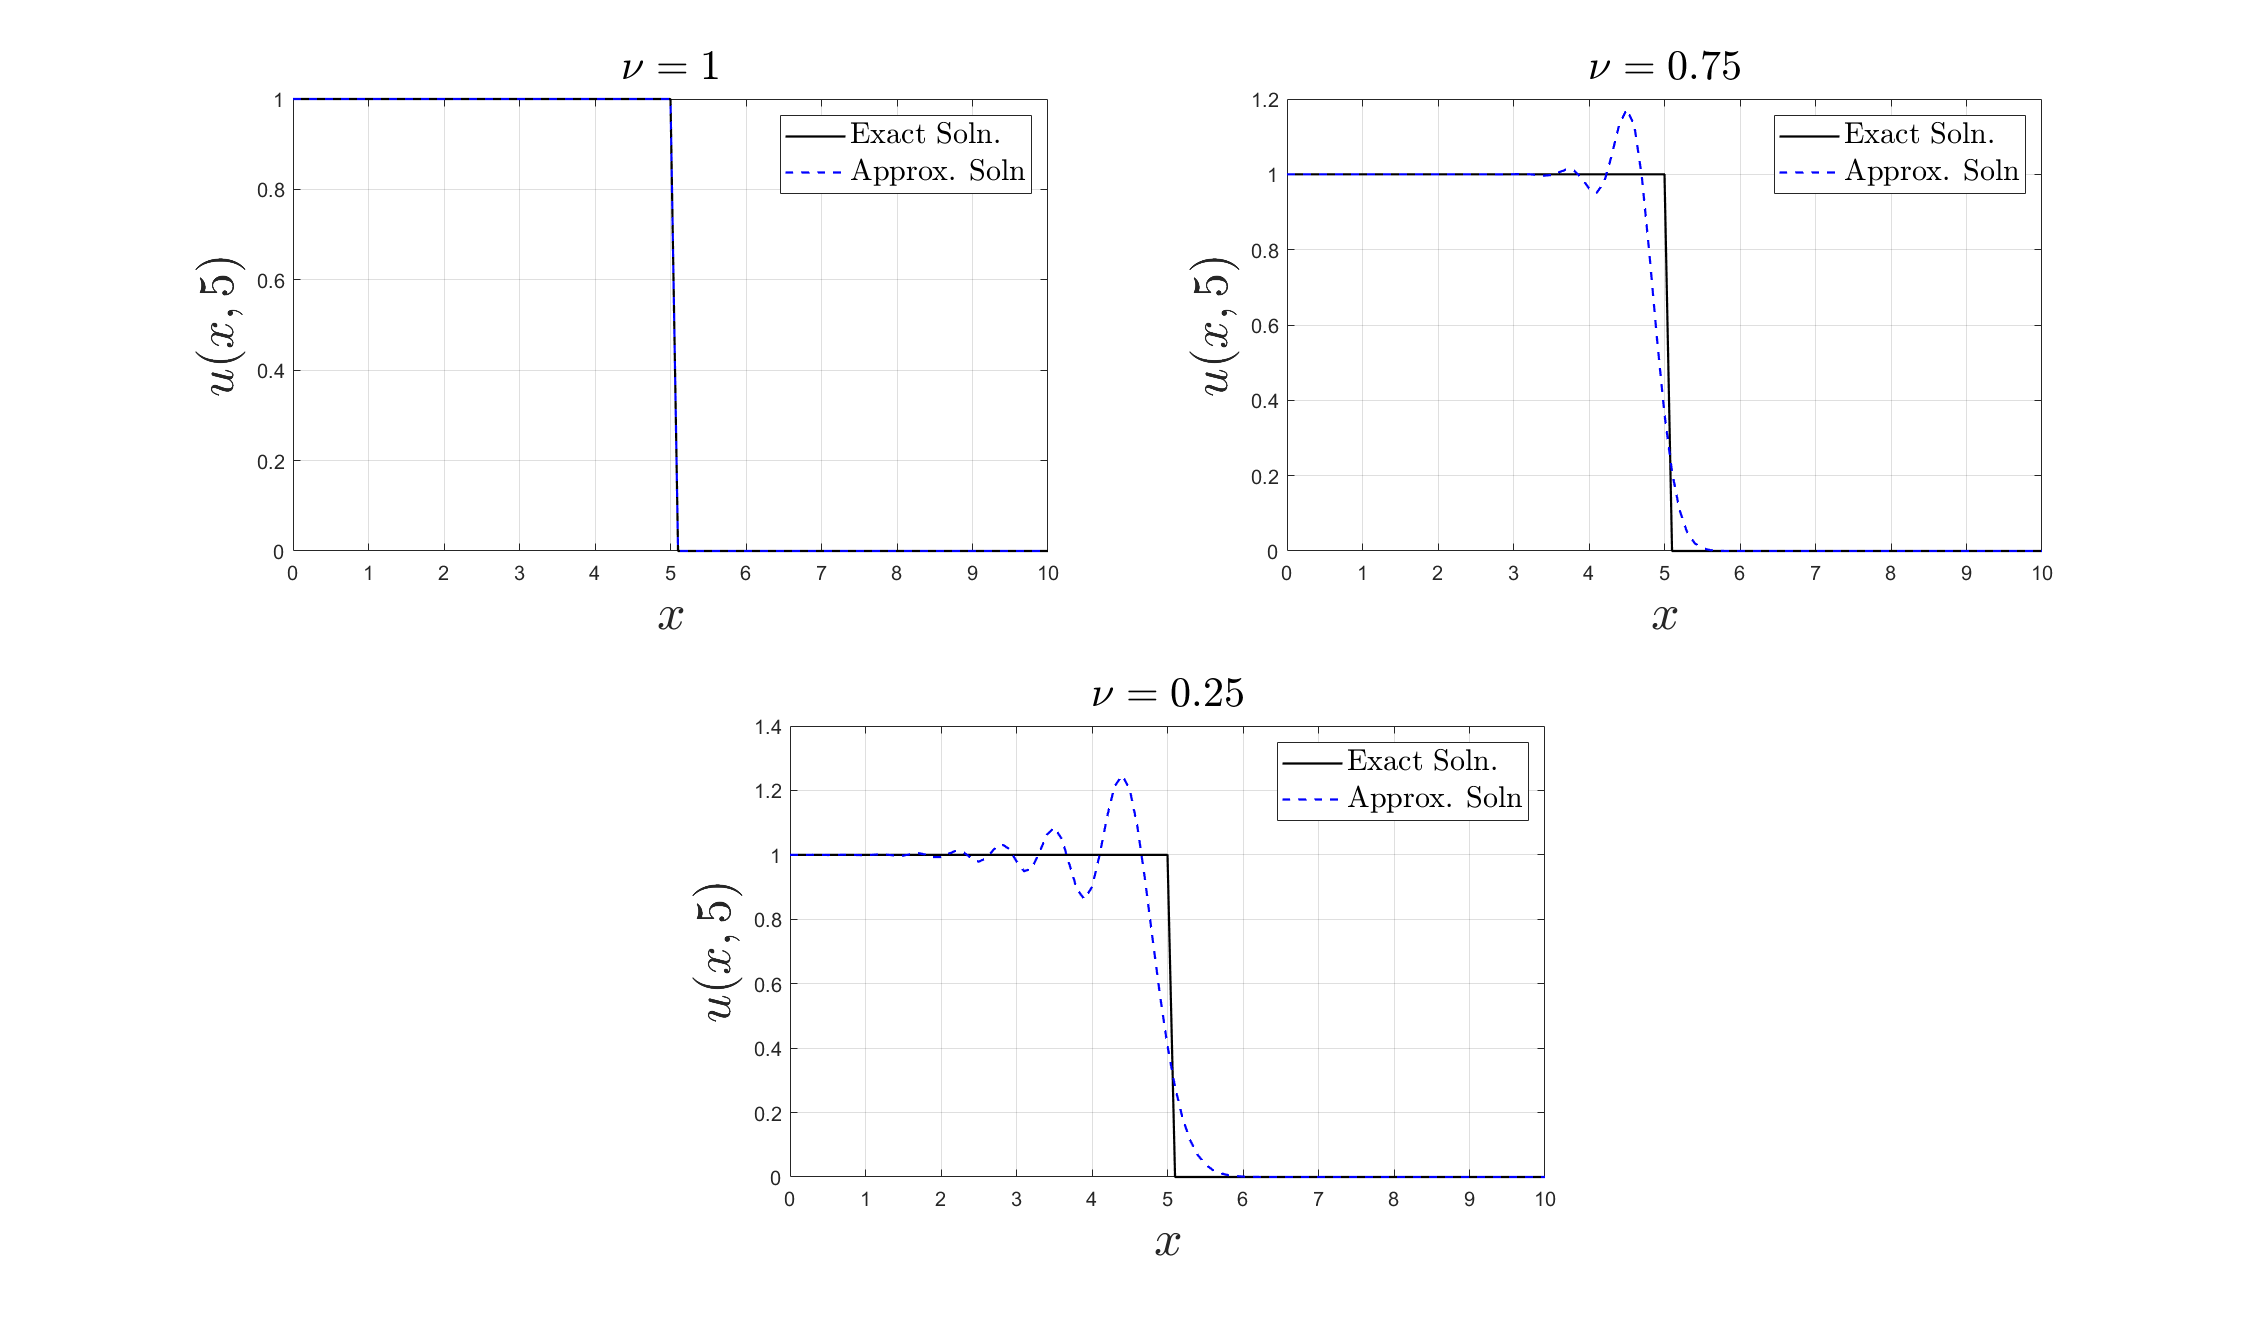
\includegraphics[scale = 0.25]{prob_3_maccormack_subplots.png}
            \end{center}
        \end{figure}
        Note that from the above figures, the Lax scheme is more diffusive than the Upwind scheme. To see why this is the case, from the modified equations in problem 2), we see that the coefficient in front of the second spatial derivative of $u$ for the upwind scheme has a $(1 - \nu)$ term while the coefficient in front of the second spatial derivative of $u$ for the Lax scheme has a $\left(\frac{1}{\nu} - \nu\right)$ term, which, when $\nu < 1$ will be greater than $1 - \nu$. That is, for $0 < \nu < 1$,
        \begin{align*}
            \nu &< 1\\
            \implies \frac{1}{\nu} &> 1\\
            \implies \frac{1}{\nu} - \nu &> 1 - \nu
        \end{align*}
        so that the diffusion coefficient for Lax is greater than the diffusion coefficient for the Upwind scheme. Further, we note that the dispersive error disappears for $\nu = 1$ since the coefficient in front of the leading terms of the modified equations for each of the schemes has $\nu = 1$ as a root. That is to say, $\nu = 1$ collapses terms on the right hand side of the modified equations, leading to the disappearance of dispersive error and improved accuracy.
    \end{itemize}
\end{itemize}

\end{document}
